\documentclass[a4paper,
fontsize=11pt,
%headings=small,
oneside,
numbers=noperiodatend,
parskip=half-,
bibliography=totoc,
final
]{scrartcl}

\usepackage{synttree}
\usepackage{graphicx}
\setkeys{Gin}{width=.6\textwidth} %default pics size

\graphicspath{{./plots/}}
\usepackage[ngerman]{babel}
%\usepackage{amsmath}
\usepackage[utf8x]{inputenc}
\usepackage [hyphens]{url}

\usepackage[colorlinks, linkcolor=black,citecolor=black, urlcolor=blue,
breaklinks= true]{hyperref}
\usepackage{booktabs} 
\usepackage[left=2.4cm,right=2.4cm,top=2.3cm,bottom=2cm,includeheadfoot]{geometry}
\usepackage{eurosym}
\usepackage{multirow}
\usepackage[ngerman]{varioref}
\setcapindent{1em}
\renewcommand{\labelitemi}{--}
\usepackage{paralist}
\usepackage{pdfpages}
\usepackage{lscape}
\usepackage{float}
\usepackage{acronym}
\usepackage{eurosym}
\usepackage[babel]{csquotes}
\usepackage{longtable,lscape}
\usepackage{mathpazo}
\usepackage[flushmargin,ragged]{footmisc} % left align footnote

\urlstyle{same}  % don't use monospace font for urls

\usepackage[fleqn]{amsmath}

%adjust fontsize for part

\usepackage{sectsty}
\partfont{\large}

%Das BibTeX-Zeichen mit \BibTeX setzen:
\def\symbol#1{\char #1\relax}
\def\bsl{{\tt\symbol{'134}}}
\def\BibTeX{{\rm B\kern-.05em{\sc i\kern-.025em b}\kern-.08em
    T\kern-.1667em\lower.7ex\hbox{E}\kern-.125emX}}

\usepackage{fancyhdr}
\fancyhf{}
\pagestyle{fancyplain}
\fancyhead[R]{\thepage}

%meta
\fancyhead[L]{E. Blumer \& K. Schuldt \\ % author
LIBREAS. Library Ideas, 24 (2014) % journal, issue, volume
\href{http://nbn-resolving.de/urn:nbn:de:kobv:11-100215863}{urn:nbn:de:kobv:11-100215863}} %urn
\fancyfoot[L] {\textit{Creative Commons BY 3.0}} %licence
\fancyfoot[R] {\textit{ISSN: 1860-7950}}

\title{\LARGE{Diese Zukunft war einmal: Ehemals moderne Bibliotheken, heute}} %title
\author{Eliane Blumer \& Karsten Schuldt} %author

\date{}
\begin{document}

\maketitle
\thispagestyle{fancyplain} 

%abstracts

%body
\section*{Planen für die Zukunft, planen für das
Scheitern}\label{planen-fuxfcr-die-zukunft-planen-fuxfcr-das-scheitern}

Wer es unternimmt, die Zukunft einer Bibliothek zu gestalten -- egal ob
als Neubau, als Um- und Anbau oder als interne Neuorganisation -- muss
einen Plan machen. Es muss sich vorgestellt werden, wie das neue Gebäude
funktionieren und aussehen soll, wem es in welcher Weise dient, wie es
eingebunden ist in sein Umfeld (der Stadt, der Schule, der Universität,
der Forschungseinrichtung, dem Bibliothekssystem). Gespeist wird dieser
Plan aus den Vorstellungen der jeweiligen Zeit, aus den jeweils
aktuellen Diskursen, aus den technischen, bibliothekstechnischen und
baulichen Möglichkeiten, aus den Debatten der aktuellen
Architekturdiskussion. Nicht zuletzt spielt die Diskussion innerhalb der
Bibliothekswesen darüber, was die Bibliothek eigentlich tun soll, eine
gewichtige Rolle. Die heutige Konzentration der Bibliothek auf die
Interessen der Nutzerinnen und Nutzer war zum Beispiel nicht immer
gegeben. Es gab Zeiten, in denen der Sammlungs- und Erhaltungsauftrag im
Mittelpunkt stand, die erzieherische Funktion von Bibliotheken als
conditio sine qua non -- gerade Öffentlicher Bibliotheken -- galt oder
die Repräsentationsfunktion von Bibliotheksgebäuden noch mehr als heute
betont wurde.

Einige anschauliche Beispiele dafür:

\begin{itemize}
\item
  Im Jahr 1954 in Leipzig im Deutsch publizierten Werk \enquote{Die
  sowjetische Massenbibliothek} nimmt der Autor W.~N. Denisjew die
  Bibliothek ganz für die bolschewistische Erziehung in Beschlag:
  \enquote{Die kulturell-aufklärenden Aufgaben der Bibliothek bestimmen
  die Rolle und die Pflichten des Bibliothekars. Es ist falsch, wenn
  manche der Ansicht sind, daß die Arbeit des Bibliothekars aus rein
  technischen Obliegenheiten besteht: ein Buch auszugeben und die
  Ausgabe im Leserformular zu vermerken, das Buch vom Benutzer wieder in
  Empfang zu nehmen und die Rückgabe zu notieren. Im Leitartikel der
  \enquote{Prawda} vom 31. August 1937 heißt es dagegen ganz richtig:
  \enquote{Der Bibliothekar ist nicht einfach ein technischer Arbeiter,
  kein mechanischer Ausgeber von Büchern. Er ist ein Propagandist und
  ein Agitator der bolschewistischen Kultur. Seine gesamte Arbeit muß
  vom Geist der bolschewistischen Ideologie und Parteilichkeit
  durchdrungen sein\ldots{} Die sowjetischen Bibliothekare stehen vor
  der großen ehrenvollen Aufgabe: den Werktätigen ihres Vaterlandes bei
  der Aneignung der bolschewistischen Kultur zu helfen, die alle besten
  Schöpfungen der Menschheit in sich birgt.} Der Bibliothekar ist
  berufen, die Bücher an die Massen heranzubringen und das Volk im
  Geiste des Sowjetpatriotismus und im Geiste der Ergebenheit an die
  Sache des Kommunismus zu erziehen. Der Bibliothekar ist ein Arbeiter
  an der ideologischen Front, er muß die Bücher und die anderen
  Druckerzeugnisse benutzen, um die überlebte bürgerliche Ideologie im
  Bewußtsein der Sowjetmenschen zu bekämpfen.} (Denisjew 1954, S. 15)
\item
  Einige Jahre später klingt dies bei Fedor Nikolaevič Paščenko, obwohl
  auch er in der Sowjetunion schrieb, ganz anders. Der politische
  Impetus ist einer funktionalistischen Beschreibung gewichen:
  \enquote{Der Bau selbständiger Gebäude für kleinere Bibliotheken geht
  in der Stadt und auch auf dem Land tendenziell zurück. Diese
  Bibliotheken werden vorwiegend in größere Mehrzweckgebäude
  eingegliedert: in der Stadt in Wohnhäuser oder
  gesellschaftlich-kulturelle Zentren, auf dem Lande in Klub- oder
  Kulturhäuser. Die Ursachen für diese Tendenz bei der Unterbringung der
  Bibliotheken liegen vor allem in städtebaulichen Überlegungen sowie im
  Bemühen um größtmöglichen Komfort für die Nutzer. Das Streben nach
  optimalen Funktionsbedingungen für die Bibliotheken ist für alle
  sozialistischen Länder charakteristisch. Die Bereitstellung neuer,
  komfortabler Räume nach neuen technischen und ästhetischen
  Gesichtspunkten ist eine überall anzutreffende Erscheinung.} (Paščenko
  \& Schwarz 1986, S. 12) Diese Verschiebung im Diskurs lässt sich mit
  den Veränderungen im politischen System der Sowjetunion erklären. Die
  politischen Veränderungen einer Zeit schlagen sich offenbar auch in
  der Sicht auf die Bibliothek nieder.
\item
  Ein anderes, an die heutigen Diskussionen in Deutschland und der
  Schweiz erinnerndes Beispiel, ist die begeisterte Darstellung des
  dänischen Öffentlichen Bibliothekswesens durch Gertrud Seydelmann:
  \enquote{Die Öffentlichen Bibliotheken Dänemarks verstehen sich heute
  nicht nur als Institute zum Lesen und Entleihen von Büchern, sondern
  als Kulturzentren, in denen die Bürger aller Alters- und
  Bildungsstufen, beim Vorschulalter beginnend bis zum bettlägerigen,
  hilfsbedürftigen alten Menschen, Information, Anregung, Bildung durch
  die verschiedensten Medien finden. Die Bibliotheken sind Kontakt- und
  Begegnungsort. Sie tragen dem durch die Vielfalt ihrer Räume Rechnung,
  die neben den Ausleihflächen, Gruppenräume, Studienzellen,
  Mehrzwecksäle, Diskothek und nicht zuletzt auch eine Cafeteria mit
  Raucherlaubnis umfassen.} (Seydelmann 1973, 10) Hieraus ergeben sich
  folgende bauliche Merkmale: \enquote{Die vielschichtige
  Aufgabenstellung für die voll ausgebaute Biblio-Mediathek erzwingt ein
  großes Bauvolumen in eigenständigen Gebäuden. Durch ihre Größe und
  ihre verschiedenartigen Funktionen sowie durch die Tradition ihrer
  Dienstleistungen sind sie fest im Bewußtsein der Bevölkerung
  verankert. Hinzu kommt die erheblich kleinere Einwohnerzahl der Städte
  im Vergleich zur Bundesrepublik, so daß die Flächenausdehnung
  überschaubar ist und sich um ein breiter gestreutes gewachsenes
  Zentrum konzentriert. Daraus ergibt sich die für deutsche
  Bibliothekare verblüffende Situation, daß neue Bibliotheksgebäude
  durchaus nicht immer im Zentrum, sondern am Rande von Verkehrs- und
  Einkaufsflächen angesiedelt sind. Sie liegen an einem kleinen See, in
  einem Park in harmonischer, nicht hektischer Umgebung.} (Seydelman
  1973, 10f.) Auffällig, dass diese Text aus den 1970er Jahren heute
  immer noch als neu gelten könnte. Offenbar bewegen sich die Debatten
  um moderne Bibliotheken nicht beständig vorwärts.
\item
  Xavier Fabre und Vincent Speller skizzieren für die Öffentlichen
  Bibliothek in Frankreich drei Phasen, in denen unterschiedlich über
  diese gedacht wurde: \enquote{Trois modèles ont marqué l'évolution
  archtiecturale des bibliothèques publiques: l'espace de conservation
  des livres et du savoir (Ètienne-Louis Boullée, projet de bibliothèque
  publice des Capucines, 1784 {[}\ldots{}{]}: les gardins des livres
  sous une voûte unique), l'espace de la lecture savante, montrant
  l'élaboration des savoirs (Henri Labrouste, grand salle de la
  Bibliothèque nationale, 1854-1875: les tables de lecture sous les
  voûtes multiples), l'espace étende du supermarché du livre derriére
  ses façades vitrées (modèle de l'accessibilité du livre à tous, et de
  la diversité des genres\ldots{}).} (Farbe \& Speller 2012, S. 54)
\end{itemize}

Diese Vorstellungen schlagen sich mal mehr, mal weniger in Zahlen und
Modellen konkretisiert, in bibliothekarischen Richtlinien wieder, wobei
an diesen im Rückblick nicht so sehr die konkreten Werte interessant
sind, sondern der Fakt, dass sie sich selber ständig verändern und in
der Realität der Bibliotheken nur zum Teil beachtet werden. Hinzu kommen
das Selbstverständnis der Bibliothek und der jeweils Planenden, ganz zu
Schweigen von den Vorstellungen der Auftraggeber. Aus all dem entsteht
ein Konglomerat, welches im Plan vom jeweils neuen, modernen
Bibliotheksbau in die Zukunft verlängert werden soll.

Alles ist veränderlich: Personen wechseln ihre Posten oder gehen in
Rente, gesellschaftliche Systeme verändern sich, die bibliothekarische
und die architektonische Diskussion betont neue Grundsätze, die
technischen Möglichkeiten verändern sich, was bibliothekstechnisch als
klug galt, gilt vielleicht -- oft aus guten Gründen -- nach einigen
Jahren als schlecht. Aber: Die einmal geplanten Gebäude stehen, wenn sie
gebaut werden, da und müssen, wohl oder übel, genutzt werden. Sicherlich
können sie anders ausgestattet werden, geplante Zonen anders genutzt
werden als vorgesehen und so weiter. Aber die grundsätzlichen
architektonischen Entscheidungen strukturieren diese Gebäude weiter.
Zehn Jahre, zwanzig Jahre, manchmal über hundert Jahre stellen sie in
Grundzügen immer noch die Arbeitsplätze von Bibliothekarinnen und
Bibliothekaren dar. Die Frage, die uns in diesem Beitrag bewegt ist, was
aus den Plänen der Bibliotheksbauten der vergangenen Dekaden wird, wenn
sie einmal umgesetzt sind.

\begin{figure}[htbp]
\centering
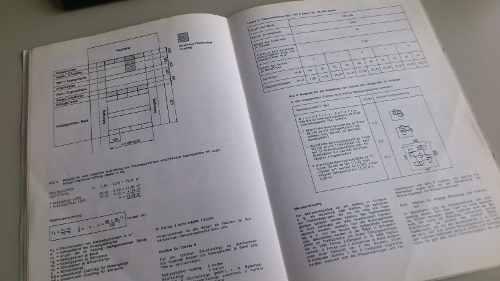
\includegraphics{./img/001.jpg}
\caption{Eines von zahlreichen Beispielen für Richtlinien und Planungen
im Bibliotheksbereich, hier aus der DDR. (Wirth 1985).}
\end{figure}

\section*{Wie plant man eine neue
Bibliothek?}\label{wie-plant-man-eine-neue-bibliothek}

Wie so eine Planung unternommen werden soll, ist eine immer wieder
umstrittene Frage. Gilt heute wohl die Beachtung der Interessen der
Nutzerinnen und Nutzer sowie eine Anlage der Bibliothek als flexibler
Raum als unabdingbar, sprechen sich in den frühen 1980er Jahren
Bibliotheksarchitekten explizit gegen diese Interessen als alleinige
Richtschnur aus:

\begin{quote}
``Feststellung von Bedarf aufgrund von empirischen Ermittlungen ergibt
noch keine relevanten Planungsgrößen, denn empirische Ermittlungen
werden nie voraussetzungslos begonnen; wir machen uns abhängig von den
Instrumenten unserer Beobachtungen, die immer -- selbst bei einfachsten
Feststellungen -- durch theoretische Voraussetzungen geprägt sind.
\end{quote}

\begin{quote}
Allgemeiner gesagt konstituieren sich Zwecke (der Bedarf) immer
innerhalb des Systems, sie werden nicht etwa von außen auferlegt, wie es
uns Bedarfsuntersuchungen vortäuschen möchten. Zwecke haben die Aufgabe,
Außenprobleme in die Dispositionsmöglichkeiten des Systems zu verlagern.
Zweckorientierung befreit so von allzu direktem Umweltdruck und
vereinfacht die Entscheidungssituation.
\end{quote}

\begin{quote}
Betrachten wir also eine Bibliothek als System, können wir es planerisch
nur erfassen, wenn wir für diese Zweckbetrachtung einen Außenbezug
herstellen, wir nach der Funktion von Zwecken fragen. Die Funktion der
Zwecke liegt nicht etwa in ihrer jeweiligen Erfüllung im Einzelzweck,
sondern ist als strategische Leistung zu sehen. {[}\ldots{}{]}
\end{quote}

\begin{quote}
Nicht der Zweckcharakter der Bibliothek, sondern die Erwartungsstruktur
der Umwelt ist die maßgebende Bezugsgröße der Entwicklung. Hier liegt
ein Kernproblem für die Planung. {[}\ldots{}{]}
\end{quote}

\begin{quote}
Der architektonische Entwurf muß in der sinnfälligen Entwicklung von
Außen- und Innenraum, in der differenzierten Folge von unterscheidbaren
Raumgruppen und vor allem in der Kongruenz von Handlungsablauf und
Raumentwicklung primäre Leitmerkmale bilden. Diese Forderung
widerspricht einer anderen Grundforderung der heutigen
Bibliotheksplanung, nämlich undifferenzierte flexible Bibliotheksräume
anzubieten. {[}\ldots{}{]}
\end{quote}

\begin{quote}
Allgemeine Zwecke sind nicht planbar. Flexibilität kann kein
Planungszweck sein. Zwecke müssen präzis formuliert werden, nur auf
diesem Weg kann eine Innendifferenzierung des Systems, die Voraussetzung
für Anpassungsfähigkeit ist, entstehen. Wenn ein spezielles
Planungsproblem möglichst gründlich und von allen Seiten her
durchgearbeitet ist, wird in der jeweils besonderen Lösung die darin
abgearbeitete und aufgehobene Problemkomplexität aller Flexibilität
überlegen sein." (Ramcke 1981, S. 63ff.)
\end{quote}

Der schon genannte Fedor Nikolaevič Paščenko gibt uns sogar eine
Anweisung für Architekt und Bibliothekar an die Hand, die hier
vollständig wiedergegeben werden soll, da sie schnell zur Einsicht
führt, wie sehr zeitgenösssischer Diskurs und Vorstellungen vom Planen
einer Bibliothek Hand in Hand gehen.

\begin{quote}
\begin{enumerate}
\def\labelenumi{\arabic{enumi}.}
\setcounter{enumi}{0}
\itemsep1pt\parskip0pt\parsep0pt
\item
Der Architekt muß fachlich kompetent sein, seine Aufgabe ernst
nehmen, Geduld und Zeit haben zur Lösung der Aufgabe, wenn notwendig, in
einigen Varianten, ein guter Zuhörer sein, seinen Standpunkt klar
formulieren können sowie Entscheidungen erst nach Konsultationen mit
anderen treffen.
\end{enumerate}
\end{quote}

\begin{quote}
\begin{enumerate}
\def\labelenumi{\arabic{enumi}.}
\setcounter{enumi}{1}
\itemsep1pt\parskip0pt\parsep0pt
\item
  Der Architekt muß willens und in der Lage sein, die Bedürfnisse des
  Auftraggebers zu interpretieren, alle Vorgaben des Auftraggebers
  einschließlich der städtebaulichen Einordnung kennen, zur Aufstellung
  eines guten Programmes beitragen und exakte Baupläne vorlegen.
\end{enumerate}
\end{quote}

\begin{quote}
\begin{enumerate}
\def\labelenumi{\arabic{enumi}.}
\setcounter{enumi}{2}
\itemsep1pt\parskip0pt\parsep0pt
\item
  Der Architekt muß primäre Wünsche des Auftraggebers funktionell und
  ästhet\-isch umsetzen, dabei die Funktionsanforderungen integrieren und
  ein nach außen und innen harmonisches Ganzes schaffen.
\end{enumerate}
\end{quote}

\begin{quote}
\begin{enumerate}
\def\labelenumi{\arabic{enumi}.}
\setcounter{enumi}{3}
\itemsep1pt\parskip0pt\parsep0pt
\item
  Der Architekt muß eine kostengünstige Variante vorlegen, dabei sind
  die Investionskosten ein genau so wichtiger Faktor wie die
  Betriebskosten.
\end{enumerate}
\end{quote}

\begin{quote}
\begin{enumerate}
\def\labelenumi{\arabic{enumi}.}
\setcounter{enumi}{4}
\itemsep1pt\parskip0pt\parsep0pt
\item
  Der Architekt benötigt einen Mitarbeiterstab proportional zur Größe
  der betreffenden Aufgabe, dabei müssen alle Beteiligten
  zusammenwirken, um ein optimal funktionierendes Gebäude dem Nutzer zu
  übergeben.
\end{enumerate}
\end{quote}

\begin{quote}
\begin{enumerate}
\def\labelenumi{\arabic{enumi}.}
\setcounter{enumi}{5}
\itemsep1pt\parskip0pt\parsep0pt
\item
  Der Architekt muß, auch wenn er schon genug Erfahrung im
  Bibliotheksbau hat, sich über die letzten Neuheiten auf dem Gebiet der
  Architektur, der Ausstattung, und Ausrüstung der Bibliotheken auf dem
  Laufenden halten und nicht nur auf sein Routine vertrauen.
  {[}\ldots{}{]}
\end{enumerate}
\end{quote}

\begin{quote}
\begin{enumerate}
\def\labelenumi{\arabic{enumi}.}
\itemsep1pt\parskip0pt\parsep0pt
\item
  Der Bibliothekar muß Funktionen und Aufgaben des neuen Gebäudes bis
  ins Detail klären und erläutern können, sich gegebenenfalls von
  herrschenden Vorstellungen und Meinungen trennen und neue Ideen und
  Vorschläge aufgreifen können, Gedanken an das alte Gebäude aus dem
  Spiel lassen, frühzeitig beginnen, Fakten zu sammeln.
\end{enumerate}
\end{quote}

\begin{quote}
\begin{enumerate}
\def\labelenumi{\arabic{enumi}.}
\setcounter{enumi}{1}
\itemsep1pt\parskip0pt\parsep0pt
\item
  Der Bibliothekar muß sich vom neuen Gebäude genaue Vorstellungen
  verschaffen, um mitreden und mitdiskutieren und dadurch mitgestalten
  zu können; er ist der Autor des Programms, das er -- mit anderen
  abgestimmt -- zu vertreten hat.
\end{enumerate}
\end{quote}

\begin{quote}
\begin{enumerate}
\def\labelenumi{\arabic{enumi}.}
\setcounter{enumi}{2}
\itemsep1pt\parskip0pt\parsep0pt
\item
  Der Bibliothekar muß lernen, daß Bibliotheksbau keine abwegige
  Nebenbe\-schäf\-tigung ist, sondern eine primäre Leitungsaufgabe von hohem
  Rang, auch über die eigene Bibliothek hinaus; der Bibliotheksbau ist
  eine gesellschaftliche Investition von hohen Kosten, er zeugt von der
  Anerkennung der Bibliotheken und des bibliothekarischen Berufs.
\end{enumerate}
\end{quote}

\begin{quote}
\begin{enumerate}
\def\labelenumi{\arabic{enumi}.}
\setcounter{enumi}{3}
\itemsep1pt\parskip0pt\parsep0pt
\item
  Der Bibliothekar muß sich für Architektur, Bauwesen und Technik im
  allgemeinen interessieren und ein aufgeschlossener Partner sein; er
  muß lernen, Pläne zu lesen und die Erklärung darauf zu verstehen, um
  rechtzeitig auf Fehler hinweisen zu können.
\end{enumerate}
\end{quote}

\begin{quote}
\begin{enumerate}
\def\labelenumi{\arabic{enumi}.}
\setcounter{enumi}{4}
\itemsep1pt\parskip0pt\parsep0pt
\item
  Der Bibliothekar muß den Architekten in die Probleme der
  Bibliothekswissenschaft und Informatik einführen, soweit diese sich im
  Bibliotheksneubau widerspiegeln und muß auch in der Lage sein,
  Einzelheiten \enquote{in der Sprache des Architekten} erläutern zu
  können.
\end{enumerate}
\end{quote}

\begin{quote}
\begin{enumerate}
\def\labelenumi{\arabic{enumi}.}
\setcounter{enumi}{5}
\itemsep1pt\parskip0pt\parsep0pt
\item
  Der Bibliothekar muß schon in der Ausbildung mit Problemen des Baus
  und der Einrichtung von Bibliotheken vertraut gemacht werden.
\end{enumerate}
\end{quote}

\begin{quote}
\begin{enumerate}
\def\labelenumi{\arabic{enumi}.}
\setcounter{enumi}{6}
\itemsep1pt\parskip0pt\parsep0pt
\item
  Der Bibliothekar muß seine Mitarbeiter regelmäßig über den
  Bibliotheksbau informieren und sie in allen Phasen in die Vorbereitung
  einbeziehen, da das Personal die Güte des späteren Baus bestimmt.
\end{enumerate}
\end{quote}

\begin{quote}
\begin{enumerate}
\def\labelenumi{\arabic{enumi}.}
\setcounter{enumi}{7}
\itemsep1pt\parskip0pt\parsep0pt
\item
  Der Bibliothekar muß die Entwicklungsrichtungen des
  wissenschaftlich-technischen Fortschritts gut kennen, den
  Möglichkeiten gemäß mit Modernisierung und Umorganisierung schon im
  alten Gebäude beginnen und von all diesen Vorhaben den Architekten
  informieren. (Paščenko \& Schwarz 1986, S. 342f.)
\end{enumerate}
\end{quote}


\section*{Dokumente und Gebäude}\label{dokumente-und-gebuxe4ude}

Manchmal hinterlassen die Pläne und Planungen mehr, als nur die Gebäude.
Sie hinterlassen Dokumente, Artikel, Festschriften, in denen dargelegt
wird, wie sich die zukünftige Bibliothek, die zukünftige Arbeit in
dieser Einrichtung gedacht wurde. Sie zeigen zum Teil auch auf, warum
bestimmte Entscheidungen getroffen wurden. In einem solchen, glücklichen
Fall lassen sich damalige Planung und heutige Realität miteinander
vergleichen.

Im Folgenden haben wir dies an einer Reihe von Bibliotheken in der
Schweiz, Österreich und Deutschland unternommen. Alle hier abgebildeten
Bibliotheken galten zum Zeitpunkt ihres Baus als modern. Die
Impressionen wurden im Sommer und Herbst 2013 (Schweiz und Deutschland)
sowie Winter 2014 (Wien) aufgenommen. Einige der Bibliotheken waren
explizit eingebunden in Diskussionen um die nationale Repräsentation
(die Schweizerische Nationalbibliothek -- ehemals Landesbibliothek --
mit ihrer zurückhaltenden Moderne, welche die Schweiz in den 1930er
Jahren, im Vorgang der Geistigen Landesverteidigung auszeichnete, oder
die Staatsbibliothek Preußischer Kulturbesitz, Berlin, Potsdamer Platz,
die sich in das geplante Kulturforum einfügt als Sinnbild eines
liberalen und offenen, kulturell geprägten Deutschlands, wie es in den
1960er und 1970er Jahren gezeichnet und auch in anderen
Repräsentativbauten wie dem Kanzlerbungalow sichtbar wurde). Andere
sollten die Stadt, in der sie sich befinden, repräsentieren und
verweisen heute oft auf eine vergangene Sicht auf diese Städte (Palais
Rumine, Lausanne; Zentralbibliothek Zürich, Zürich;
Amerika-Gedenkbibliothek, Berlin). Wieder andere zeigen den Versuch,
Lösungen im kleinen Raum zu finden und berichten von vergangenen (eigene
Bibliothekscontainer wie in Spiez) oder aktuellen Methoden (An- und
Umbau an vorhandene Gebäude wie in Münsingen). Einige Bauten
hinterlassen nichts ausser Spuren in den Archiven und
Bibliotheksbeständen. Dies muss nicht immer heissen, dass die
Bibliotheken gänzlich verschwinden. Das aktuelle Gebäude der
Bezirksbibliothek Berlin-Köpenick ist zum Beispiel dort errichtet, wo in
den 1980er Jahren ein anderes Bibliotheksgebäude errichtet wurde.

Was kann aus den Gegenüberstellungen gelernt werden? Sicherlich zwei
Dinge: Zum einen scheitern alle Pläne mit der Zeit. Einige -- sicherlich
die meisten -- scheitern im Planungsprozess der Ausführung und werden
nie gebaut.~ Ein schönes Beispiel dafür ist der Architekturwettbewerb
zum Umbau der Amerika-Gedenkbibliothek in Berlin in den späten 1980er
Jahren. (Feireiss, 1989) Dieser Umbau sollte die effektiv nutzbare
Fläche der Bibliothek erweitern, an den schon einmal modernen Bau der
1950er Jahre anschliessen sowie den Blücherplatz -- den Standort der
Bibliothek -- räumlich neu erschliessen. Der Wettbewerb war weit
fortgeschritten, genauer: abgeschlossen. Es wurden sogar die Preise für
die ersten Plätze verteilt und eine Publikation mit den
Wettbewerbsbeiträgen gedruckt (Feireiss 1989). Gleichwohl: mit dem Jahr
1989 und der politischen Wende trat ein neues Projekt auf den Plan. Die
Amerika-Gedenkbibliothek (West) wurde mit der Stadtbibliothek Berlin
(Ost) zur Zentralen Landesbibliothek Berlin zusammengeführt. Diese
strebt seitdem einen gemeinsamen Neubau an. (Lux 2011) Deshalb wurde das
Gebäude der Amerika-Gedenkbibliothek nicht mehr verändert. Dem Karneval
der Kulturen -- einem der etablierten jährlich stattfindenden
Strassenfeste in Berlin -- geriet das zum Vorteil, da heute der gesamte
Blücherplatz und der daran anschliessende Park für das jährliche Fest
genutzt werden kann. Die fertigen architektonischen Entwürfe allerdings
haben die Zeit ihrer Umsetzung offenbar hinter sich gelassen.

Aber dies ist nicht das einzige mögliche Scheitern. Auch gebaute
Entwürfe scheitern mit der Zeit. Die Vorstellungen, die mit ihnen
verbunden wurden, werden mit der Zeit überholt. Die weiter unten
stehenden Bilder legen davon Zeugnis ab. So haben sich Vorstellungen
einer auf Ewigkeiten planbaren Bibliothek, wie sie zum Beispiel im
Palais Rumine, Lausanne, zu finden sind, als haltlos erwiesen. Auch der
Bibliothekscontainer in Spiez zeugt eher von einer nicht mehr
vertretenen Vorstellung, nach der Bibliotheken als eigenständige
Einrichtung möglichst separat gebaut eingerichtet werden sollten. Die
technisch weit überholten Internetstationen, die bis zum Herbst 2013 in
der Amerika-Gedenkbibliothek, Berlin, genutzt wurden, zeigen zudem, dass
Entwicklungen nicht alle gleich schnell verlaufen. Das Gebäude, immerhin
mehrere Jahrzehnte alt, erscheint nicht so unmodern wie die zum
Zeitpunkt des Bildes vielleicht zehn Jahre alten -- und in zwischen
ausgetauschten -- Stationen.

\begin{figure}[htbp]
\centering
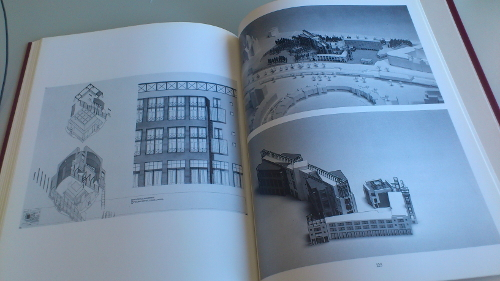
\includegraphics{./img/002.jpg}
\caption{Pläne zum Umbau der Amerika-Gedenkbibliothek, Berlin (Feireiss
1989).}
\end{figure}

\begin{figure}[H]
\centering
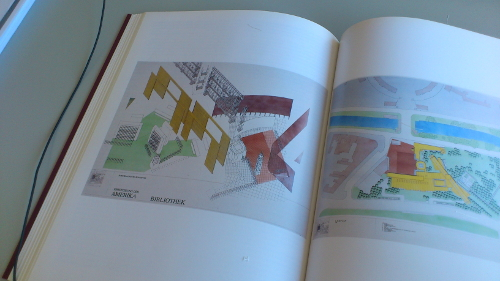
\includegraphics{./img/003.jpg}
\caption{Pläne zum Umbau der Amerika-Gedenkbibliothek, Berlin(Feireiss
1989).}
\end{figure}

Zudem: Trotz diesem Scheitern der ehemaligen Pläne funktionieren alle
diese Gebäude auch heute als öffentliche Räume, zumeist immer noch als
Bibliotheken. Es wurden zum Teil grosse bauliche Veränderungen
durchgeführt, die Arbeitsabläufe um die Gegebenheiten herum organisiert,
Kompromisse wurden eingegangen. Und bestimmt haben die Kolleginnen und
Kollegen in allen Häusern Vorstellungen, wie es besser zu organisieren
wäre. Aber: Neubauten sind selten. Ein gescheiterter Plan heisst nicht,
dass das gesamte System Bibliothek scheitert.

\section*{Ehemals Moderne Bibliotheken. Dokumente und
Situationen}\label{ehemals-moderne-bibliotheken.-dokumente-und-situationen}

\subsection*{Schweizerische Nationalbibliothek (Bern,
Schweiz)}\label{schweizerische-nationalbibliothek-bern-schweiz}

\begin{quote}
\enquote{Durch den Haupteingang betritt man Windfang und Vorraum, von wo
breite Gänge, die wechselnden Ausstellungen dienen können, rechts und
links nach den Seitenflügeln mit den verschiedenen Ämtern führen,
während geradeaus, durch Glastüren sofort sichtbar, sich Bücherausgabe
und Lesesall der Bibliothek befinden. Grosser Lesesaal,
Zeitschriftensaal, Bücherausgabe, Warteraum und Katalogsaal bilden einen
grossen gemeinsamen Raum, dessen Abteilungen nur durch Glaswände
abgetrennt sind. Dadurch gewinnt der beaufsichtigende Beamte die beste
Übersicht und der Besucher das Gefühl der Weiträumigkeit. Auf die
übliche Galerie für die Handbibliothek ist verzichtet, dafür besitzt
dieser Saal nussbaumgetäferte Nischen, die die Handbibliothek aufnehmen.
Die obere Wandzone des Saales ist mit Akustik-Celotex verkleidet, dessen
schalldämpfende Wirkung sich sehr stark fühlbar macht, und der ausserdem
als Material eine sehr symphatisch weiche, rauhe Oberfläche hat. Der
grosse Saal wie auch der Katalogsaal, der Ausstellungssaal und das
Karten- und Bilderzimmer empfangen ihr Tageslicht ausschliesslich von
oben, dagegen besitzt der grosse Lesesaal in seiner äussersten, den
Zeitschriften reservierten Abteilung westliches Seitenlicht, da sich die
ganze Stirnwand des Saales gegen den Garten im Westen öffnet. Hier
lagert sich dem Saal eine geräumige, nach aussen offene gedeckte
Terrasse vor, die dem Besucher der Bibliothek den Aufenthalt auch bei
längerer Dauer angenehm machen und ihm Gelegenheit zur Entspannung im
Freien geben soll. Ein Fresco von Ernst Morgenthaler an der Schmalwand
dieser Loggia ist der einzige bildliche Schmuck des Gebäudes, denn man
hat mit Bedacht davon abgesehen, die mit Celotex bekleideten, oberen
Wandzonen des grossen Saales mit bildblichen Darstellungen
auszuschmücken, die die Aufmerksamkeit des Lesenden für sich in Anspruch
nehmen, also von der Lektüre ablenken würden. Es ist zu hoffen, dass
sich die neuartige Idee, der Bibliothek einen solch offenen Raum und
Austritt in den Garten beizugeben, bewähren wird.} (Anonym 1931, S.7f.)
\end{quote}

\begin{quote}
\enquote{Das ganze Gebäude bekommt seine besondere Straffheit der
Komposition dadurch, dass alle Abmessungen als gemeinsames Mass die
Axendistanz der Bücherregale enthalten. Sie beträgt im Büchermagazin
1,52 m und ist dort unmittelbar an den enggereihten schmalen Pfeilern
der Fassade abzulesen.} (Anonym 1931, S. 8)
\end{quote}

\begin{quote}
\enquote{Begreiflicherweise haben die äusseren Formen der neuen
Landesbibliothek nicht überall Zustimmung gefunden. Der Verzicht auf
klassische oder sonst ornamentale Architekturformen wirkt noch immer auf
jene Betrachter befremdlich, die sich nicht Rechenschaft geben, dass
damit die Freiheit gewonnen wurde, das Gebäude nach der Seite seiner
praktischen Benutzbarkeit um so besser durchzubilden.} (Anonym 1931, S.
12f.)
\end{quote}

\begin{quote}
\enquote{Es darf als besonderer Glückfall bezeichnet werden, dass der
Neubau in einer bei staatlichen Gebäuden seltenen Kompromisslosigkeit
durchgeführt werden konnte.} (Anonym 1931, S. 18)
\end{quote}

\begin{quote}
\enquote{Das Gebäude der Landesbibliothek war 1927-1931 grosszügiger
geplant und gebaut worden, als es die damaligen Platzansprüche
verlangten. Vier Bundesämter, das Eidg. Amt für geistiges Eigentum, das
Eidg. Statistische Amt, das Eidg. Inspektorat für Forstwesen, Jagd und
Fischerei sowie die Eidg. Getreideverwaltung wurden als eine Art Puffer
in den Büroflügeln einquartiert und sollten im Laufe der Zeit der
wachsenden Bibliothek weichen. Dieses Konzept erwies sich allerdings nur
während einiger Jahrzehnte als befriedigend. Zwar sind nach wie vor
genügend Büroflächen verfügbar, und ein Teil der Räume wurde inzwischen
vom Bundesamt für Kultur und vom Schweizerischen Literaturarchiv
übernommen. Dagegen fanden wegen der Flut neuer Publikationen
schliesslich nur noch etwa ein Drittel der Bestände im Büchermagazin
Platz. Ausserdem stellten die Bibliothekare neue Ansprüche an die
Konservierung wertvoller Bücher und an die Logistik des Betriebs.}
(Allenspach \& Schibig 2001, S. 5)
\end{quote}

\begin{quote}
``Der Landesbibliothek haften die Merkmale einer Übergangssituation an:
Die Architekten suchten nach neuen Konzepten, taten dies aber nicht mit
letzter Konsequenz. Eine ähnliche Tendenz kann gleichzeitig bei anderen
Neubauten in der Schweiz beobachtet werden, so beim Börsengebäude in
Zürich, gebaut 1929-30 von Henauer \& Witschi, bei den Berner Bauten von
Salvisberg um 1930 und kurz danach beim Bau von Gewerbeschule und
Kunstgewerbemuseum in Zürich durch Karl Egender und Adolf Steger von
1930-33.
\end{quote}

\begin{quote}
Die Landesbibliothek war ein modernistischer Kompromiss und lag viel
stärker im Zeitgeist als die ebenfalls 1927 entstandenen, provokativen
Entwürfe eines Le Corbusier und von Hannes Meyer und Hans Wittwer für
den Völkerbundpalast in Genf. Alfred und Heinrich Oeschger standen nicht
mit den avantgardistischen Kreisen der Schweizer Architektur in
Verbindung und wurden 1930 auch nicht zum damaligen Grossereignis, dem
Bau der Woba-Siedlung in Basel des Schweizerischen Werkbundes
eingeladen. Der zurückhaltende Modernismus will indes nicht bedeuten,
dass die Architektur keine kohärenten gestalterischen Qualitäten
besässe. Ganz im Gegenteil hat die sorgfältige Rennovation erneut die
grossen Qualitäten eines Werkes sichtbar gemacht, das vom Gesamtentwurf
bis zu den Details der Gestelle und Leuchten mit innerer Überzeugung und
Talent geplant und ausgeführt wurde." (Allenspach \& Schibig 2001, S.
60f.)
\end{quote}

\begin{figure}[htbp]
\centering
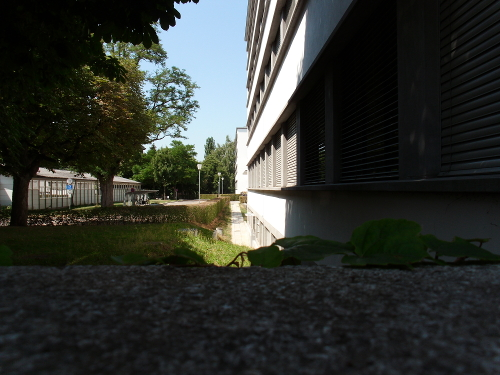
\includegraphics{./img/004.jpg}
\caption{Schweizerische Nationalbibliothek (Bern,
Schweiz)}
\end{figure}

\begin{figure}[htbp]
\centering
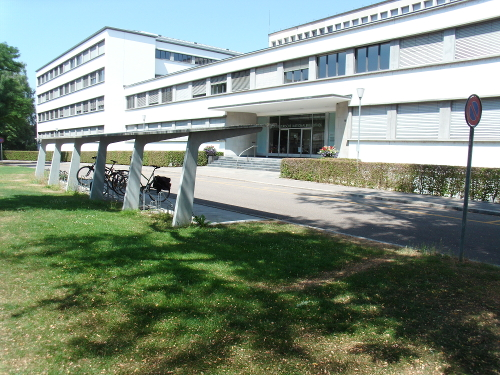
\includegraphics{./img/005.jpg}
\caption{Schweizerische Nationalbibliothek (Bern,
Schweiz)}
\end{figure}

\begin{figure}[htbp]
\centering
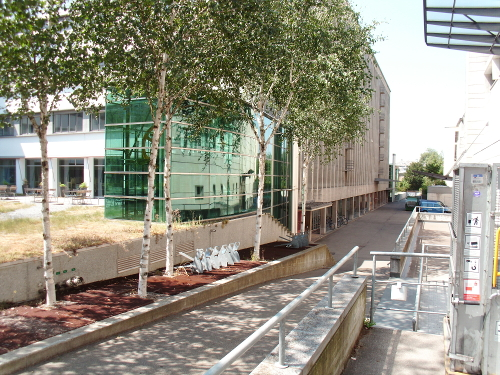
\includegraphics{./img/006.jpg}
\caption{Schweizerische Nationalbibliothek (Bern,
Schweiz)}
\end{figure}

\begin{figure}[htbp]
\centering
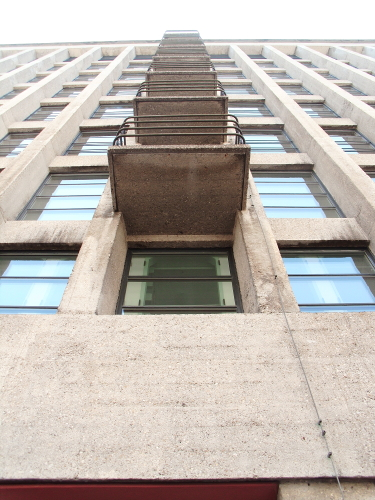
\includegraphics{./img/007.jpg}
\caption{Schweizerische Nationalbibliothek (Bern,
Schweiz)}
\end{figure}

\begin{figure}[htbp]
\centering
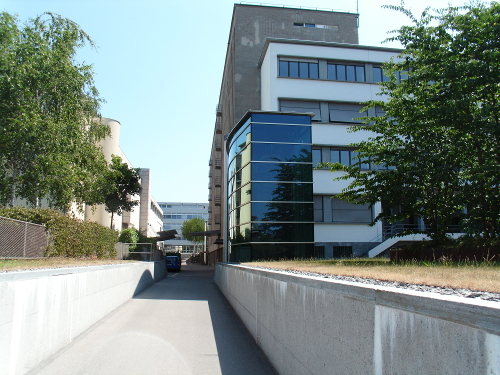
\includegraphics{./img/008.jpg}
\caption{Schweizerische Nationalbibliothek (Bern,
Schweiz)}
\end{figure}

\subsection*{Staatsbibliothek Preussischer Kulturbesitz (Berlin,
Deutschland)}\label{staatsbibliothek-preussischer-kulturbesitz-berlin-deutschland}

\begin{quote}
\enquote{Der große Kubus des Hauptlesesaals wurde zum Pavillon der
Nationalgalerie versetzt angeordnet und die entstehende Flankenbeziehung
durch den weit vorstoßenden molenkopfartigen Kubus des Vortragssaals
exponiert, der gliedernd die Raumbildung im Bereich der Potsdamer Straße
bewirkt. Die städtebauliche Beziehung des Pavillons der Nationalgalerie
geschieht über eine vorgelagerte Skulpturenterasse und terrassenartig
ansteigende Flachbauten des Ibero-Amerikanischen Instituts zu dem
Lesesaal mit den Sonderabteilungen. Die peripheren zwei- und
viergeschossigen Randbauteile mit dem Ibero-Amerikanischen Institut oder
dem Institut für Bibliothekstechnik im Norden, die allseits das Bauwerk
umgeben, sind in ihrer Dimensionierung zugleich maßstabgeben für die
höheren Baukörper und für die beginnende Parklandschaft des Tiergartens;
sie bewirken den angestrebten menschlichen Maßstab des Bauwerks.}
(Wisniewski 1978, S. 150)
\end{quote}

\begin{quote}
\enquote{Der Raum zum Lesen darf nicht trennen, nicht spezialisieren,
sondern das Angebot dem Lesen darlegend -- letztlich demokratisch -- die
Auswahl gewährleisten. So sollte auch das Gebäude dieses Angebotes nicht
formaler, irisierender Selbstzweck werden, sondern unbegrenzt und
richtungslos wie eine Landschaft, tendenzlos sein.} (Wisniewski 1978, S.
154f.)
\end{quote}

\begin{quote}
\enquote{Die Eingangshalle hat {[}\ldots{}{]} die Funktion eines
Verteilers. Man gelangt von hier sowohl in den internen Bereich der
Bibliothek als auch zu dem im gleichen Baukomplex untergebrachten
Ibero-Amerikanischen Institut und dem Vortragssaal. Der \enquote{Ort der
Begegnung} in der Eingangshalle bildet zugleich die Einstiegsstelle für
das Leit- und Informationssystem, das dem Benutzer die Orientierung im
öffentlichen Bereich erleichtert.} (Drozd 1978, S. 179)
\end{quote}

\begin{quote}
``Die bibliothekarische Organisationsplanung hat sich stets von dem
Grundsatz leiten lassen, daß es sich bei diesem Gebäude um eine Bauwerk
von hohem architektonischen Rang handelt, dem die ihm angemessene
bibliothekarische Funktion gegeben werden muß; diese darf der
architektonischen Konzeption zwar nicht zuwiderlaufen, muß jedoch den
Bedürfnissen einer wissenschaftlichen Bibliothek entsprechen.
\end{quote}

\begin{quote}
Alle Bemühungen der Planungen um eine Funktionalität dieses
Bibliotheksgebäudes werden in Zukunft auch daran gemessen werden,
inwieweit das Haus flexibel genug ist, um sich an neue, heute noch nicht
vorhersehbaren Aufgaben anzupassen. Die Qualität des architektonischen
Entwurfs wird sich in Zukunft gerade bei solchen Anforderungen bewähren
müssen." (Drozd 1978, S. 183)
\end{quote}

\begin{figure}[htbp]
\centering
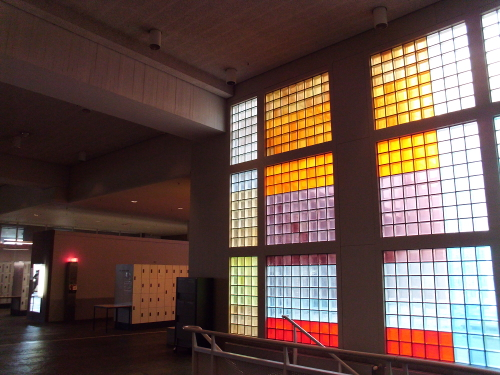
\includegraphics{./img/009.jpg}
\caption{Staatsbibliothek Preussischer Kulturbesitz (Berlin,
Deutschland)}
\end{figure}

\begin{figure}[htbp]
\centering
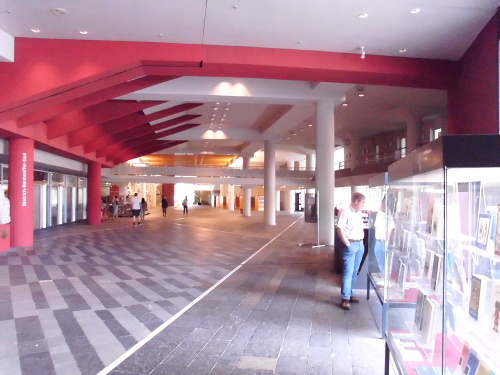
\includegraphics{./img/010.jpg}
\caption{Staatsbibliothek Preussischer Kulturbesitz (Berlin,
Deutschland)}
\end{figure}

\begin{figure}[htbp]
\centering
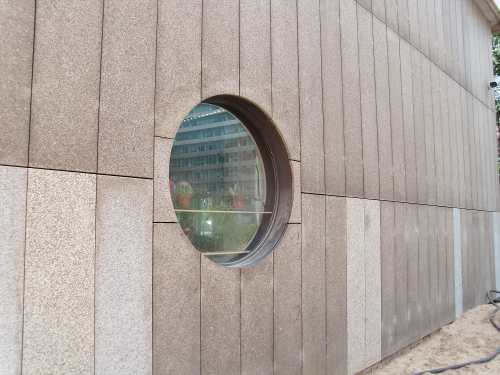
\includegraphics{./img/011.jpg}
\caption{Staatsbibliothek Preussischer Kulturbesitz (Berlin,
Deutschland)}
\end{figure}

\begin{figure}[htbp]
\centering
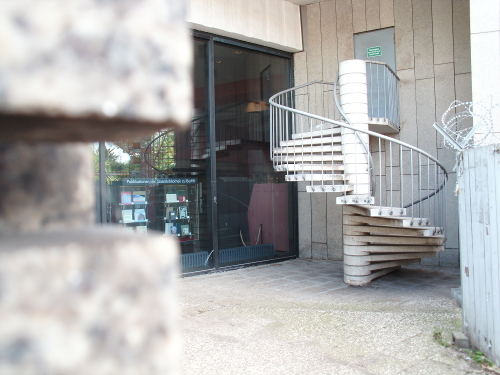
\includegraphics{./img/012.jpg}
\caption{Staatsbibliothek Preussischer Kulturbesitz (Berlin,
Deutschland)}
\end{figure}

\begin{figure}[htbp]
\centering
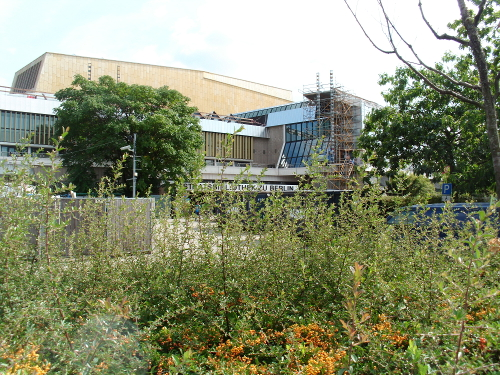
\includegraphics{./img/013.jpg}
\caption{Staatsbibliothek Preussischer Kulturbesitz (Berlin,
Deutschland)}
\end{figure}

\subsection*{Palais Rumine (Lausanne,
Schweiz)}\label{palais-rumine-lausanne-schweiz}

\begin{quote}
``Unter der Leitung des Ingenieurs Samuel de Mollins fanden beim Bau des
Palais de Rumine die neusten Techniken jener Zeit Anwendung. Fundament,
Fenster- und Türstürze sowie die Dachbalken wurden nach dem
Hennebique-Prinzip aus Stahlbeton erstellt. Grösstenteils jedoch wurden
jene Materialien eingesetzt, die für öffentliche Bauten Ende des 19.
Jahrhunderts in der Westschweiz üblich waren: Der Sockeln besteht aus
Kalkstein von St.~Triphon, die rustikalen Bossen der Grundmauern aus
Arvel-Stein. Die Bossen der oberen Stockwerke, die Eckquarder und das
Gefüge der Hauptfassade bestehen aus Villebois-Kalkstein, ebenso der
Beckenrand des Brunnens im Atrium und die Passage über die lange
Eingangstreppe. Für die oberen Stockwerke wurde bleicher Kalkstein von
Savonnières und Morley verwendet. Die beiden grossen Säulen vor dem
Palais bestehen aus rosafarbenem Granit von Baveno und die
Kolonnadenreihe aus Kalkstein von Villebois. Für gewisse Details wurden
speziellere Materialien eingesetzt: schottischer Granit für die
Cabochons an der Westfassade, Gotthard-Gneiss für die Haupttreppe,
Mont-Blanc-Granit für die Treppe zur Rue Pierre-Viret, Hauteville-Stein
für die Säulen des Eingangsportals und den Sockel über dem Becken des
Atriums, Stein aus Echaillon für die Doppelsäulen der oberen Galerie und
die Handläufe der Ehrentreppe.
\end{quote}

\begin{quote}
{[}\ldots{}{]}
\end{quote}

\begin{quote}
Der Grossteil des Schmucks befindet sich in den Durchgangsbereichen, die
zusätzlich mit Kunstschmiedearbeiten von Louis Fatio aus Lausanne und
Mosaiken von Mathieu Pedroli aus La Tour-de-Peilz ausgestattet wurden.
In den Ausstellungssälen hingegen blieb die Dekoration nüchtern und
bestand meist aus monochromem Stuck. Einzig der grosse Saal der
Bibliothek wurde mit figurativen Wandmalereien und mit Steinimitationen
ausgeschmückt.
\end{quote}

\begin{quote}
{[}\ldots{}{]}
\end{quote}

\begin{quote}
Am 3. November 1906 fand schliesslich die feierliche Einweihung des
Palais de Rumine statt. Das Budget war allerdings um 40 Prozent
überschritten worden, und die einzelnen Institutionen fühlten sich von
Anfang an eingeengt. Die Zahl der Studierenden {[}der Universität
Lausanne{]} hatte sich in der Tat innerhalb von zehn Jahren verdoppelt
und stieg von 600 im Jahr 1896 auf 1200 im Jahr 1906 an. Auch die
Bibliothek litt bereits unter Platznot." (Corthésy 2008, S. 15f.)
\end{quote}

\begin{quote}
\enquote{Während beinahe des ganzen 20. Jahrhunderts und selbst bis in
unsere Tage hinein zeugten gewisse Initiativen von einer Unbeliebtheit
dieses Baus, dessen Masslosigkeit in Grösse und Ausschmückung von der
Bevölkerung von Lausanne mehrheitlich abgelehnt wurde.} (Corthésy 2008,
S. 17)
\end{quote}

\begin{quote}
\enquote{Das Palais de Rumine beherbergt zahlreiche, sehr
unterschiedliche Institutionen, deren Ziele und Bedürfnisse einem
ständigen Wandel unterzogen sind. Deshalb ist heute schon abzusehen, das
dem Bauwerk noch zahlreiche Veränderungen bevorstehen. Für die nächsten
Jahre sind in der Tat wichtige Neuerungen vorgesehen, den Parlament und
Kunstmuseum ziehen in eigens für sie erstellte Gebäude. Die
verschiedenen vorgenommenen Umbauarbeiten sind von unterschiedlicher
Qualität und reichen von tief greifenden Massnahmen bis zu respektvollem
Umgang mit dem historischen Bau, dessen Gesamteindruck indessen nie
unwiederbringlich verändert wurde.} (Corthésy 2008, S. 49)
\end{quote}

\begin{figure}[htbp]
\centering
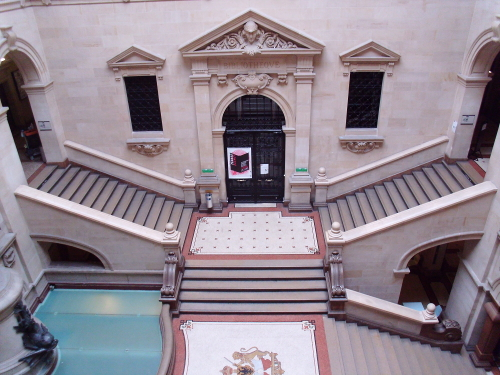
\includegraphics{./img/014.jpg}
\caption{Palais Rumine (Lausanne,
Schweiz)}
\end{figure}

\begin{figure}[htbp]
\centering
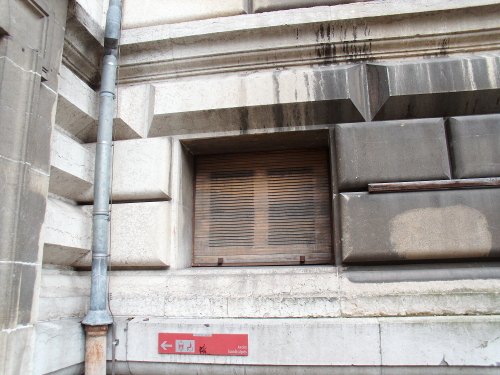
\includegraphics{./img/015.jpg}
\caption{Palais Rumine (Lausanne,
Schweiz)}
\end{figure}

\begin{figure}[htbp]
\centering
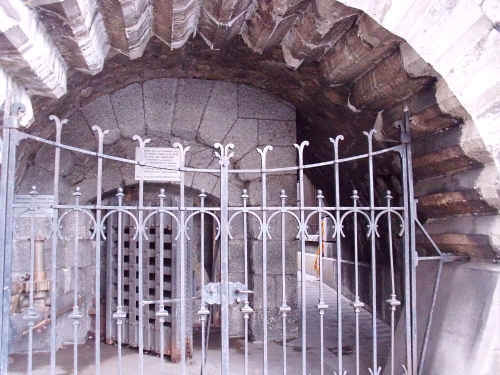
\includegraphics{./img/016.jpg}
\caption{Palais Rumine (Lausanne,
Schweiz)}
\end{figure}

\begin{figure}[htbp]
\centering
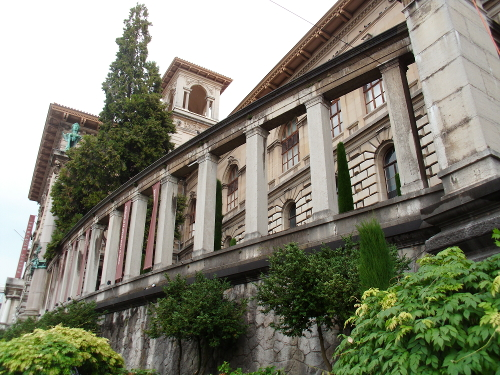
\includegraphics{./img/017.jpg}
\caption{Palais Rumine (Lausanne,
Schweiz)}
\end{figure}

\begin{figure}[htbp]
\centering
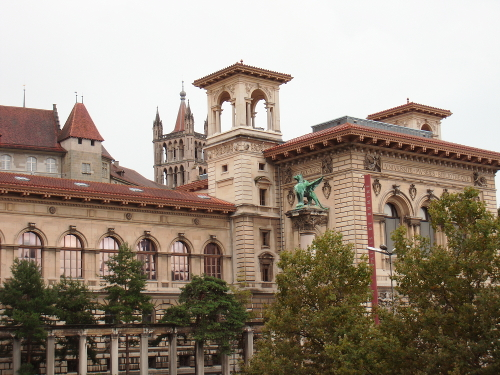
\includegraphics{./img/018.jpg}
\caption{Palais Rumine (Lausanne,
Schweiz)}
\end{figure}

\subsection*{Zentralbibliothek Zürich (Zürich,
Schweiz)}\label{zentralbibliothek-zuxfcrich-zuxfcrich-schweiz}

Zum Bau der Zentralbibliothek in Zürich, 1914 in einer Abstimmung vom
Volk beschlossen, hat sich ein anonymes Gedenkblatt erhalten, dass hier,
wegen seines Werts als zusammenhängende Darstellung und Begründung des
Baus, vollständig zitiert wird. Seit dieser Zeit wurde das Gebäude, zu
einem Grossteil unterirdisch, mehrfach ergänzt.

\begin{quote}
``I. Allgemeines
\end{quote}

\begin{quote}
Die Zentralbibliothek ist erwachsen aus der Gegenbewegung gegen die im
Laufe der Zeit eingetretene Zersplitterung des zürcherischen
Bibliothekswesens, die dadurch entstanden war, daß sich neben der im
Jahre 1629 gegründeten Stadt- (oder Bürger-) Bibliothek zunächst drei
kleinere Bibliotheken (die der naturforschenden Gesellschaft, der
medizinisch-chirurgischen Bibliotheksgesellschaft und der juristischen
Bibliotheksgesellschaft) und sodann im Jahre 1835 die mit ihren ältesten
Bestände auf die Stiftsbibliothek des Großmünsters zurückgehende
Kantonsbibliothek, auch Bibliothek der kantonalen Lehranstalten genannt,
bildeten. Seit 1896 von verschiedenen Seiten angeregt, seit 1897 von der
Stadtbibliothek offiziell angestrebt, wurde die Vereinigung der beiden
Hauptbibliotheken im Sommer 1902 entscheidend gefördert durch die
Schenkung eines hochherzigen Gönners im Betrage von 200.000 Fr. an den
Kanton. Mehrjährige Verhandlungen zwischen den beidseitigen Behörden
führten die verwickelten Fragen zu einer beide Teile befriedigenden
Lösung, die am 1. März 1914 durch Volksabstimmung von der städtischen
Einwohnerschaft, am 28. Juni gleichen Jahres von der des Kantons
gutgeheißen wurde. Zwei Probleme galt es im Wesentlichen zu lösen: das
der Errichtung und Finanzierung des erforderlichen Neubaus und das der
organischen Gestaltung der darin unterzubringenden Sammlungen.
\end{quote}

\begin{quote}
Als organische Form -- um zunächst von dieser zu sprechen -- wurde, da
eine Abtretung der einen Bibliothek an den Eigentümer der anderen
ausgeschlossen war, die einer von Kanton und Stadt gemeinsam errichteten
Stiftung gewählt, für deren Bedürfnisse, erstmalige wie künftige, die
Stifter aufzukommen haben. Rechte und Pflichten wurden gleichmäßig
verteilt. Jeder Teil ernennt in die Stiftungsbehörde gleichviele
Mitglieder und trägt an den Aufwand der Anstalt gleichviel bei. Immerhin
wurden die beidseitigen Sammlungsbestände ungewertet eingeworfen, da
eine Wertung mit zu großen Schwierigkeiten verbunden gewesen wäre. Die
Stiftungsbehörde kann sich, abgesehen davon, daß sie auf die jeweiligen
beidseitigen Zuschüssen angewiesen ist und den beiden Stiftern Bericht
und Rechnung zu erstatten hat, in ihren Entscheidungen frei bewegen.
\end{quote}

\begin{quote}
Für den Bau wurde ein der Stadt gehörender und von ihr einzuwerfender
Platz bestimmt, der aus vier dafür ins Auge gefaßten schließlich als
einziger übrig blieb, auf dem sich die Interessen des Kantons und der
Stadt vereinigten. Als Gegenwert überwies der Kanton das daran
anstoßende, bis anhin die Kantonsbibliothek beherbergende, mit neuem
Einbau zu versehende Predigerchor. Ermöglicht wurde der Bau und damit
das Zustandekommen der ganzen Bibliothekvereinigung überhaupt durch
freiwillige Gaben im Betrag von nahezu 800,000 FR., die, dank einer
außergewöhnlichen Opferwilligkeit, außer dem bereits erwähnten Gönner,
eine Anzahl hiesiger und auswärtiger Private und Firmen spendete.
\end{quote}

\begin{quote}
\begin{enumerate}
\def\labelenumi{\Roman{enumi}.}
\setcounter{enumi}{1}
\itemsep1pt\parskip0pt\parsep0pt
\item
  Der Neubau
\end{enumerate}
\end{quote}

\begin{quote}
Moderne Bibliothekbauten {[}sic!{]} haben nach dem Ausspruch eines
englischen Fachmannes im Wesentlichen zwei Anforderungen zu erfüllen:
erstens die Bücher möglichst zusammenzudrängen, um Raum zu sparen, und
zweitens die Wege zu ihnen möglichst kurz zu halten, um Zeit zu sparen.
Als weitere Gesichtspunkte sind aufzustellen, daß sich die Wege für die
Benutzer und die für die Beschaffung der Bücher aus den Magazinen nicht
berühren, daß die hauptsächlichsten Benutzungs- und Verwaltungsräume
bequem zugänglich und wenn möglich auf gleicher Höhe liegen und daß für
die nötige Erweiterungsfähigkeit gesorgt ist, und zwar nicht nur für das
Gebäude im Ganzen, sondern für jede der beiden Raumgruppen, in die ein
Bibliothekbau {[}sic!{]} zerfällt, nämlich für die Benutzungs- und
Verwaltungsräume einesteils und für das Büchermagazin andernteils im
Besondern.
\end{quote}

\begin{quote}
Der Neubau zerfällt in drei Hauptteile: 1. den Verwaltungsbau, 2. den
Lesesaalbau 3. den Magazinbau. {[}sic!{]}
\end{quote}

\begin{quote}
Der Lesesaalbau
\end{quote}

\begin{quote}
liegt abseits vom Lärm und Staub der Straße im Zentrum der Bauanlage
zwischen den neuen Gebäudeflügeln und der Predigerkirche. Er umfaßt den
Lesesaal von 290 m2 Bodenfläche, 7,5 m lichter Höhe und 126
Arbeitsplätze, den Vortragssaal, die Bücherausgabe und den Arbeitsraum
der Abwärte. Sein Licht empfängt der Lesesaal durch ein Glasoberlicht,
das durch einen elektrisch betriebenen Vorhang gegen das direkte
Sonnenlicht und durch eine Heizanlage im Hohlraum zwischen dem
horizontalen Oberlicht und dem Glasdach gegen Verdunklung durch Schnee
geschützt ist. Ein seitliches Fenster dient hauptsächlich
Lüftungszwecken. Auch die übrigen Räume dieses Bauteils sind durch
Oberlicht beleuchtet. Der Lesessaal ist unterkellert zur Aufnahme der
Zentralheizungs- und Lüftungsanlagen und des Kohlenraumes.
\end{quote}

\begin{quote}
Die Konstruktion des Neubaues ist in allen Teilen, einschließlich das
Dach, feuersicher durchgeführt worden. Die Büchergestelle sind von Eisen
hergestellt. Die künstliche Beleuchtung geschieht durch Elektrizität,
die Beheizung im Verwaltungsbau und Lesesaal durch Warmwasser und in den
Bücherräumen durch Dampf. Für den großen Lesesaal und den
Zeitschriftenlesesaal wurde eine mechanische Lüftungsanlage mit der
Möglichkeit der Luftbefeuchtung erstellt." (Anonym 1917)
\end{quote}

\begin{figure}[htbp]
\centering
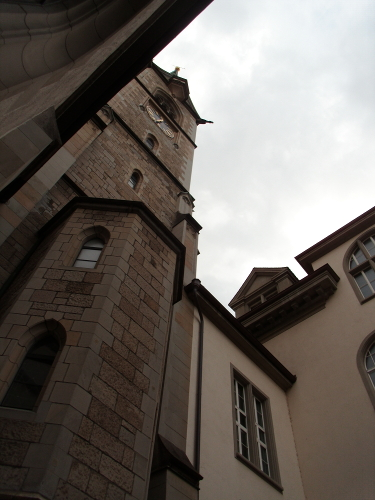
\includegraphics{./img/019.jpg}
\caption{Zentralbibliothek Zürich (Zürich,
Schweiz)}
\end{figure}

\begin{figure}[htbp]
\centering
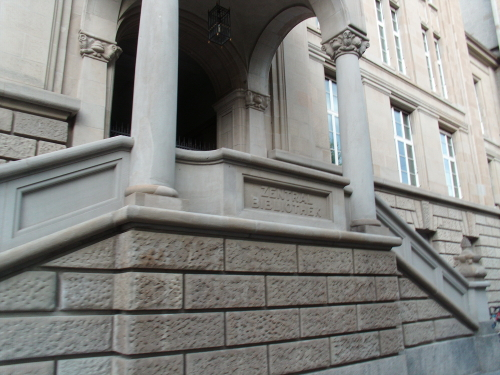
\includegraphics{./img/020.jpg}
\caption{Zentralbibliothek Zürich (Zürich,
Schweiz)}
\end{figure}

\begin{figure}[htbp]
\centering
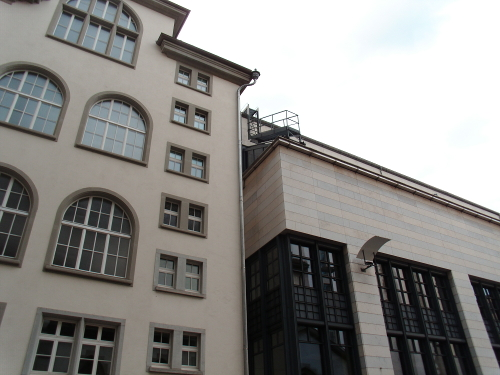
\includegraphics{./img/021.jpg}
\caption{Zentralbibliothek Zürich (Zürich,
Schweiz)}
\end{figure}

\subsection*{Amerika-Gedenkbibliothek (Berlin,
Deutschland)}\label{amerika-gedenkbibliothek-berlin-deutschland}

Die Amerika-Gedenkbibliothek ist wohl die -- zumindest in Deutsch -- am
intensivsten beschriebene Bibliothek. Der Hauptgrund ist offenbar, dass
diese Bibliothek explizit als politische Einrichtung gegründet wurde.
Die Bibliothek sollte ein Symbol des freien Berlin gegenüber der
Sowjetischen Besatzungszone darstellen. Sie stand, wie in mehreren
frühen Texten betont wird, explizit in Sichtachse der Friedrichstraße.
Die Bibliothek wird in diesen Texten auch als Ausgangspunkt der
Freihandbibliotheken in Deutschland bezeichnet, sie sollte, so die
Gründergeneration, eine Verbindung zwischen dem demokratischen
Deutschland und US-amerikanischer Kultur darstellen. (Conant 1954, Moser
1964, Anonym 1989) Im Laufe der Jahre verschwand -- einhergehend mit den
politischen Änderungen -- diese Gründungsüberlegung aus den Texten zur
Amerika-Gedenkbibliothek. Nach der politischen Wende wurde die
Bibliothek mit der Berliner Stadtbibliothek (Berlin Ost) zur Zentralen
Landesbibliothek Berlin (ZLB) vereinigt. Seitdem bemüht sich die Leitung
der ZLB um einen Neubau. (Lux 2011) Ein solcher Neubau würde, falls er
jemals umgesetzt wird, eventuell das Ende der Amerika-Gedenkbibliothek
-- und der Berliner Stadtbibliothek -- bedeuten. Dies würde immerhin für
die Bibliotheksgeschichte die Möglichkeit eröffnen, die Geschichte einer
mit Symbolik beladenen Einrichtung von Anfang bis Ende zu untersuchen.
Aktuell ist ein solches Ende, trotz abgeschlossenem
Architekturwettbewerb, nicht in Sicht.

\begin{quote}
``Für die Ausarbeitung der Entwürfe waren drei Monate Frist gesetzt. 538
Wettbewerbsunterlagen wurden angefordert und 194 Lösungen der Jury
eingereicht. 80\% der Arbeiten erfüllten den Leistungsumfang, jedoch nur
10~\% vermochten das Raumprogramm einzuhalten. Besondere Schwierigkeiten
bereitete offenbar das Nebeneinander der betrieblichen Raumfunktion. Die
Entwürfe, die in dieser Beziehung noch am meisten befriedigten, suchten
die Lösung in vielen ausgedehnten Oberlichträumen, die jedoch lange Wege
und manche Störungen durch Reparaturen, Säu\-berungen usw. befürchten
ließen.
\end{quote}

\begin{quote}
Der Schwierigkeit und Bedeutung der Aufgabe trug die Zusammensetzung des
Preisgerichts Rechnung, das nicht nur aus Berliner Experten des Bau- und
Bibliothekswesens und den Vertretern der Fachverwaltung bestand
{[}\ldots{}{]}, sondern auch namhafte westdeutsche Fachleute hinzuzog
und durch die Entsendung zweier Amerikaner unterstützt wurde. Nach
viertägigen Beratungen entschied das Preisgericht, einen 1. Preis, der
nur einer überragenden eindeutigen Lösung zuerkannt werden konnte, nicht
zu verteilen, sondern zwei Preisgruppen zu bilden und zwei gleichwertige
Arbeiten in die erste und vier weiter in die zweite Gruppe einzustufen
{[}\ldots{}{]}. Außerdem wurden 10 bemerkenswerte Entwürfe angekauft."
(Moser 1964, S. 16f.)
\end{quote}

\begin{quote}
``Mit der Errichtung der \emph{Amerika-Gedenkbibliothek} im Sinne
einer \emph{Berliner Zentralbibliothek} wurde eine der fühlbarsten Lücken
im organischen Aufbau des Berliner Bibliothekswesens geschlossen. Das
neu geschaffene Institut stellt die Brücke dar zwischen dem Unterbau der
in den Bezirken mit Bildungsaufgaben betrauten städtischen Bü\-cher\-eien
und den mannigfaltigen Bibliothekseinrichtungen, die durch ihre
Bindungen an einen enger oder weiter gezogenen Kreis wissenschaftlicher
Forschung und Lehre im Speziellen gekennzeichnet sind. Wie jene in der
Erfüllung nachbarschaftlicher Hilfeleistung ihre vornehmste Aufgabe
sehen müssen, so ist diesen aus den Ansprüchen des jeweiligen
Studienplatzes notwendig Ziel und Grenze gesteckt. Beide, für sich sehr
verschiedene Formen und Absichten der Buchvermittlung, können ein
großstädtisches Gemeinwesen schlechterdings nicht von der Notwendigkeit
entbinden, den Wünschen und Interessen aller Bevölkerungsschichten,
gleich welcher Bildungsstufe, in einem Zentrum der geistigen Berührung
eine weitgespannte Grundlage der wissenschaftlichen Unterrichtung und
Weiterbildung zu bieten.
\end{quote}

\begin{quote}
Daß diese Forderung einem echt demokratischen Antrieb entspringt, geht
schon aus der Geschichte hervor; denn etwa im gleichen Verhältnis, wie
in den modernen Kulturstaaten die souveräne Verantwortung auf das Volk
selbst überging, hat auch der verpflichtende Gedanke zur Einrichtung und
Unterhaltung solcher Bildungszentren Gestalt angenommen. Eine wichtige,
oftmals entscheidende Rolle spielten hierbei die aus privater Initiative
geborenen Bestrebungen zur Verbesserung und Verbreitung der
Volksbildung, die die Schaffung von Büchereien als eines der
unentbehrlichen Mittel zur Erreichung dieses Zieles erkannten." (Moser
1954, ohne Seite)
\end{quote}

\begin{quote}
\enquote{Eines der wichtigsten Merkmale der Bibliothek ist darin zu
erblicken, daß alle öf\-fent\-lichen Benutzerräume (mit Ausnahme der
Spezialsammlungen) zu ebener Erde liegen. Der Besucher betritt von
Norden die durch eine hohe Fensterfront erleuchtete Eingangshalle, an
deren rechter Giebelwand ein Ausspruch von Thomas Jefferson das Geleit
gibt, während linker Hand sich der Zugang zu dem Auditorium öffnet.
Neben der Kleiderablage führen Ganzglastüren in einen zweiten Vorraum,
der rechts von den Tischen für die Rücknahme der entliehenen Bücher und
die Leseranmeldung begrenzt wird. Die zurückgegebenen Bücher werden in
dem dahinter gelegenen Raum auf Vorbestellungen und Beschädigungen
durchgesehen und zur Rückbeförderung in die Freihand- und
Magazinabteilung vorsortiert. In der Leserannahmestelle werden nur
solche Benutzer registriert, die Bücher auszuleihen wünschen. Die
Benutzung des Lesesaales dagegen ist an keine Formalitäten gebunden. Auf
der linken Seite befindet sich die Ausfertigungsstelle, die nach
mechanischem Verfahren die Buchung der von dem Leser zur Ausleihe
vorgelegten Bände vornimmt. Hier werden ebenfalls die vorbestellten
Bücher ausgegeben.} (Moser 1954, ohne Seite)
\end{quote}

Der damalige Leiter der Bibliothek der ETH Zürich, Paul Scherrer, war
zur Eröffnung der A\-me\-rika-Gedenkbibliothek nach Berlin geladen. Er nahm
daran teil. Die auf dieser Reise zusammengetragenen Dokumente
(Presseaussendungen, Einladungen zu Diners, Photographien, Broschüren)
vermachte er der eigenen Bibliothek, in der sie auch heute zu finden
sind und ein interessantes historisches Dokument darstellen. Innerhalb
dieses Konvoluts findet sich auch die Rede des damaligen
US-amerikanischen Hochkommisars James B. Conant, welcher sehr eindeutig
die politische Aufgabe der Amerika-Gedenkbibliothek darstellte:

\begin{quote}
``Wir alle wissen, dass wir unsere Aufmerksamkeit nicht zu
ausschliesslich auf materielle Dinge richten duerfen, und dass der
Fortbestand Berlins als Vorposten der freien Welt nicht allein durch
eine gesunde Wirtschaft, sondern vor allem auch durch ein bluehendes
kulturelles Leben gesichert wird. Wir alle sehen mit Zuversicht dem Tage
entgegen, an dem Berlin als Hauptstadt eines in Frieden und Freiheit
wiedervereinigten Deutschlands seinen gebuehrenden Platz einnehmen wird.
Bis zu diesem Tage bleibt es die Aufgabe der freien Welt, insbesondere
der Bundesrepublik und der drei hier anwesenden Schutzmaechte, alles zu
tun, um Berlin, ein Symbol der Freiheit, zu staerken und zu
unterstuetzen, und zwar nicht nur auf wirtschaftlichem und
militaerischem, sondern auch auf geistigem Gebiet.
\end{quote}

\begin{quote}
Gerade diese Bibliothek, die so dicht an der Sektorengrenze liegt,
unterstreicht, wie wichtig in dieser Zeit voller Schwierigkeiten und
Spannungen, wie wichtig in dieser geteilten Welt die Besinnung auf die
grossen kulturellen Werte unserer freien abendlaendischen Kultur ist.
Diese Bibliothek soll die Bedeutung Berlins als eines der grossen
geistigen Widerstandszentren gegen die Unfreiheit dokumentieren. Sie
soll gleichzeitig anknuepfen an das grosse kulturelle Erbe dieser Stadt,
die schon seit Jahrhunderten solch hervorragende Rolle im geistigen
Leben Deutschlands gespielt hat." (Conant 1954, ohne Seite)
\end{quote}

\begin{quote}
``Den Vereinigten Staaten ging es ueberhaupt nicht darum, sich selbst
ein Denkmal in Berlin zu setzen, einen riesigen Adler etwa -- das
Wappentier der U.S.A. -- oder ein anderes Kolossalmonument. Was uns
vorschwebte, war eine Erinnerungsstaette fuer spaetere Generationen an
die Zeit, da das Wohl dieser Stadt ein Anliegen aller Nationen der
Freien Welt war, an die Zeit, in der Amerikaner mit den tapferen
Berlinern zusammenarbeiten und kaempfen durften, um den Wuergering der
Unfreiheit um diese Stadt zu sprengen. Wir wollten etwas von bleibendem
Wert schaffen, nicht so sehr im materiellen Sinne, sondern zum Gedenken
an den Geist dieser Stadt in den Tagen schwerster Krise. Ein
deutsch-amerikanischer Ausschuss wurde eingesetzt, dem Vertreter der
Stadtverwaltung, der Industrie, der Gewerkschaften und des
Erziehungswesens angehoerten, um ueber die zweckmaessigeste Verwendung
dieses Geldes zu entscheiden. Ich freue mich besonders, dass ihre Wahl
auf eine Bibliothek fiel.
\end{quote}

\begin{quote}
Die unnatuerliche Teilung dieser Stadt bewirkte, dass den Berlinern
keine ausreichende Zahl von Bibliotheken zur Verfügung stand. Gewiss hat
der Osten auch Bibliotheken, aber jedermann weiss, dass dort dem Leser
nur eine begrenzte, auf ein einziges totalitaeres System ausgerichtete
geistige Kost vorgesetzt wird.
\end{quote}

\begin{quote}
Zwischen den kommunistischen Bibliotheken und denen des freien Westens
besteht der gleiche Gegensatz wie zwischen einer Kultur, die auf dem
totalitaeren Autoritaetsprinzip beruht, und einer Kultur, die auf dem
Freiheitsprinzip aufgebaut ist.
\end{quote}

\begin{quote}
Solange die Ost-West-Spannung besteht, solange die Welt geteilt ist,
nicht nur in den politischen und wirtschaftlichen, sondern vor allen
Dingen auch in den kulturellen Bereichen, wird diese in Sichtweite des
unfreien Ostens gelegene Bibliothek ein Symbol fuer die Ueberlegenheit
der Freiheit des Denkens ueber den Geist der Unfreiheit sein." (Conant
1954, ohne Seite)
\end{quote}

\begin{quote}
\enquote{Gewisse unverkennbare Mängel -- etwa die Lückenhaftigkeit des
Gebotenen infolge des Absenz des Ausgeliehenen, Erschwerungen
technischer Art durch das Verstellen der Bände, eine größere Abnutzung
-- sind nicht zu bestreiten. Beim Abwägen der Vor- und Nachteile fallen
letztere jedoch um so weniger ins Gewicht, je höher der öffentliche,
allgemeinverbindliche Charakter und die gemischte, vielschichtige
Struktur der Leserschaft veranschlagt wird. Die Unvollkommenheiten der
Freihand in einem so groß gespannten Rahmen können sich freilich nur
dann in ihr positives Gegenteil verwandeln, wenn zugleich ein
Katalogwerk vorhanden ist, das über den gesamten Fundus erschöpfend
Aufschluß gibt.} (Moser 1964, S. 32)
\end{quote}

\begin{quote}
``Der erste Öffnungstag, ein Montag, übertraf die kühnsten Mutmaßungen.
Mehrmals mußte die Polizei die Pforten schließen, da es drinnen -- am
Anmeldepult und zwischen den Freihandregalen --‚ wie in einem Warenhaus
beim Sommerschlußverkauf wogte und wimmelte. Einige Pessimisten zogen
daraus sofort ihre Schlüsse und äußerten die Befürchtung, dieser
unruhige Ort würde niemals zu einer ‚Heimstätte des Geistes‛ werden.
\end{quote}

\begin{quote}
Bereits am ersten Tage wurden 2850 Bücher ausgeliehen. Zweifellos
speiste sich das gestaute Interesse zu einem beträchtlichen Prozentsatz
aus bloßer Neugier, und der Anteil der ‚Volksbüchereileser‛ war
anfänglich besonders hoch. Aber war das ein Wunder, wenn man bedenkt,
daß der Heimatbezirk Kreuzberg mit vier Büchereien und einem Bestand von
insgesamt rd. 48000 vielfach veralteten Bänden noch ganz unzureichend
versorgt war, während die AGB einen höchst attraktiven, überwiegend
neuen Bestand anbot?" (Moser 1964, S. 39)
\end{quote}

\begin{quote}
``Zur Zeit ihrer Eröffnung im Jahre 1954 war die
Amerika-Gedenkbibliothek die mit Abstand modernste Bibliothek in der
Bundesrepublik Deutschland. Dies lag daran, daß hier zum ersten Mal nach
dem Kriege ein großes neues Bibliotheksgebäude für eine öffentliche
Bibliothek nach angloamerikanischem Vorbild als \enquote{Public Library}
errichtet werden konnte.
\end{quote}

\begin{quote}
Wesentliche Neuheit war das Angebot von rund 90.000 Bänden im
Freihandbereich. So war es primär die neue Konzeption, die diese
Bibliothek zum Vorbild für alle anderen Bibliotheken der Bundesrepublik
Deutschland machte, wobei sich dies auch im Gebäude widerspiegelte."
(Anonym 1989, S. 9)
\end{quote}

\begin{figure}[htbp]
\centering
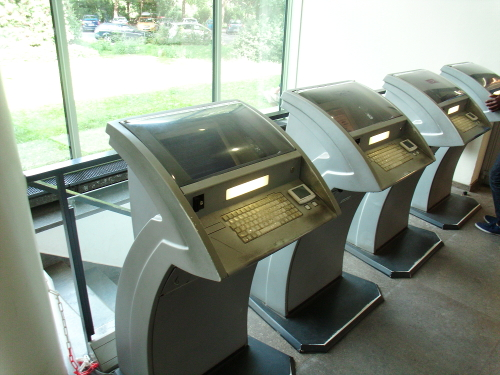
\includegraphics{./img/022.jpg}
\caption{Amerika-Gedenkbibliothek (Berlin,
Deutschland)}
\end{figure}

\begin{figure}[htbp]
\centering
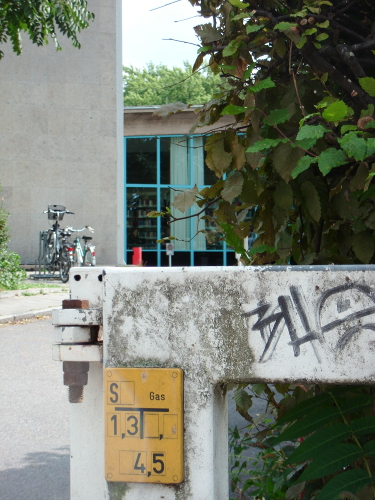
\includegraphics{./img/023.jpg}
\caption{Amerika-Gedenkbibliothek (Berlin,
Deutschland)}
\end{figure}

\begin{figure}[htbp]
\centering
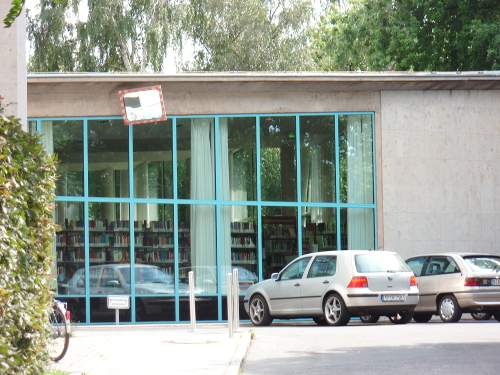
\includegraphics{./img/024.jpg}
\caption{Amerika-Gedenkbibliothek (Berlin,
Deutschland)}
\end{figure}

\begin{figure}[htbp]
\centering
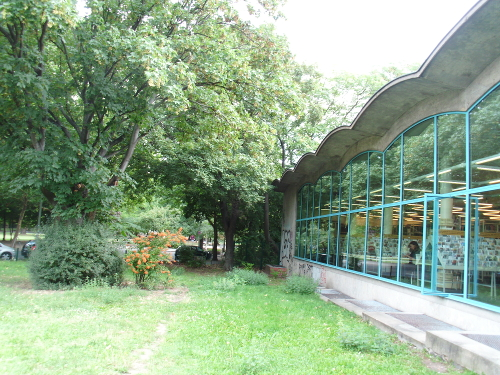
\includegraphics{./img/025.jpg}
\caption{Amerika-Gedenkbibliothek (Berlin,
Deutschland)}
\end{figure}

\begin{figure}[htbp]
\centering
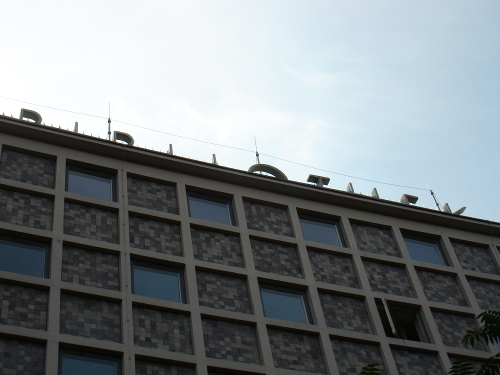
\includegraphics{./img/026.jpg}
\caption{Amerika-Gedenkbibliothek (Berlin,
Deutschland)}
\end{figure}

\begin{figure}[htbp]
\centering
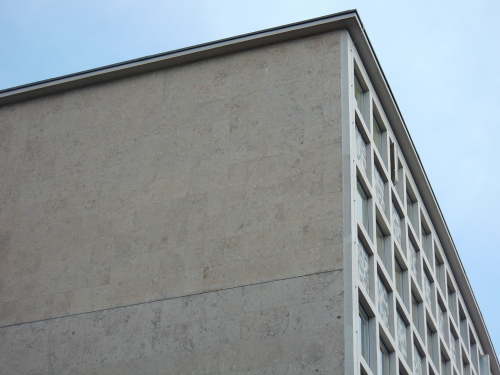
\includegraphics{./img/027.jpg}
\caption{Amerika-Gedenkbibliothek (Berlin,
Deutschland)}
\end{figure}

\subsection*{Haus des Buches, Wiener Städtische Büchereien (Wien,
Österreich). Jetzt: Musikschule
Wien}\label{haus-des-buches-wiener-stuxe4dtische-buxfcchereien-wien-uxf6sterreich.-jetzt-musikschule-wien}

\begin{quote}
\enquote{Die städtebauliche Absicht der Architekten war die Erreichung
einer Auflockerung im eng verbauten VIII. Gemeindebezirk. Deshalb wurde
das Studentenheim als optischer Abschluss in einen 33 m hohen, leicht
gekurvten Hochhausteil zusammengefasst und davor das nur zweigeschossige
Haus des Buches in Form eines abgestumpften Dreieckes um einen
sechseckigen Innenhof herum angeordnet.} (Jaksch, Fischer \& Kroller
1986, S. 134)
\end{quote}

\begin{quote}
\enquote{Der Bücherei fehlt ein größerer zusammenhängender Lesebereich
(insbesondere im Winter, wenn das Atrium nicht verwendbar ist). Es wäre
daher zu überlegen, diesen Innenhof mit einem Glasdach zu versehen und
zu schließen. Auch der Bereich der Anmeldung, Information, Bücherausgabe
und Ausleihe erscheint zu karg bemessen und sollte etwas abgeschlossener
sein, um den darin arbeitenden Personen mehr Ruhe und
Konzentrationsmöglichkeit bieten zu können.} (Jaksch, Fischer \& Kroller
1986, S. 134)
\end{quote}

\begin{figure}[htbp]
\centering
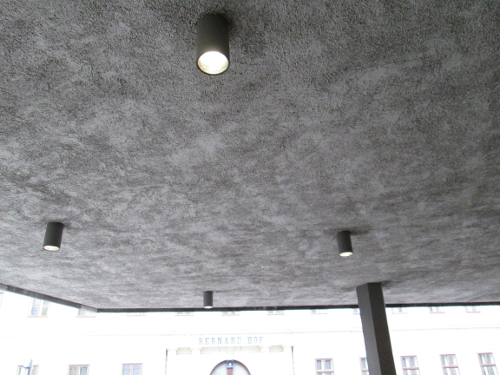
\includegraphics{./img/028.jpg}
\caption{Haus des Buches, Wiener Städtische Büchereien (Wien,
Österreich). Jetzt: Musikschule
Wien}
\end{figure}

\begin{figure}[htbp]
\centering
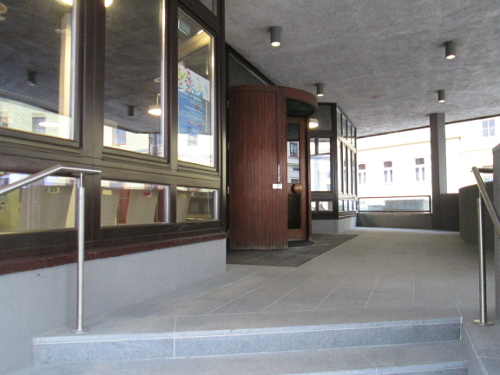
\includegraphics{./img/029.jpg}
\caption{Haus des Buches, Wiener Städtische Büchereien (Wien,
Österreich). Jetzt: Musikschule
Wien}
\end{figure}

\begin{figure}[htbp]
\centering
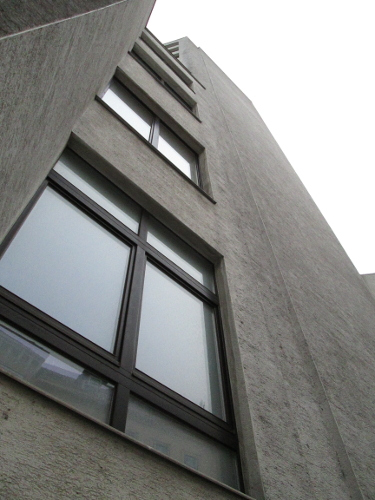
\includegraphics{./img/030.jpg}
\caption{Haus des Buches, Wiener Städtische Büchereien (Wien,
Österreich). Jetzt: Musikschule
Wien}
\end{figure}

\begin{figure}[htbp]
\centering
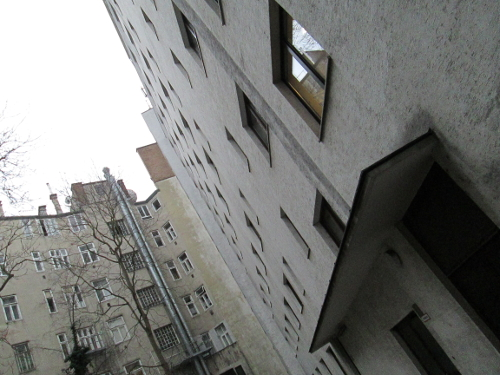
\includegraphics{./img/031.jpg}
\caption{Haus des Buches, Wiener Städtische Büchereien (Wien,
Österreich). Jetzt: Musikschule
Wien}
\end{figure}

\begin{figure}[htbp]
\centering
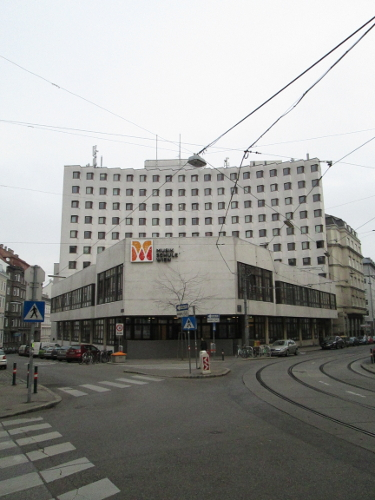
\includegraphics{./img/032.jpg}
\caption{Haus des Buches, Wiener Städtische Büchereien (Wien,
Österreich). Jetzt: Musikschule
Wien}
\end{figure}

\subsection*{Universitätsbibliothek Stuttgart (Stuttgart,
Deutschland)}\label{universituxe4tsbibliothek-stuttgart-stuttgart-deutschland}

\begin{quote}
\enquote{In seiner Eröffnungsrede lobte Bibliotheksdirektor Manfred
Koschlig den bauleitenden Architekten Klaus-Jürgen Zabel, er habe sich
in die Denk- und Vorstellungswelt der Bibliothekare eingedacht, weshalb
die Funktionsabläufe einer Bibliothek von der Akquise bis zur Ausleihe
optimiert sind. Freilich mussten auf beiden Seiten Kompromisse
eingegangen werden. Knackpunkte in Stuttgart sind die großzügige
Durchfensterung und vor allem die Südausrichtungen des Hauptlesesaals,
die vom Wunsch nach dem Bezug vom Inneren ins Grün das Stadtgartens
getragen waren und auf der negativen Seite eine zu hohe
Sonneneinstrahlung verursachten. Der Kompromiss bestand aus einer Reihe
von Sonnenschutzmaßnahmen: An der Ost- und Westseite wurden
Aluminium-Rollstores angebracht, die außen vor den Scheiben laufen und
über je einen Elektromotor angetrieben werden sind. Die Südseite erhielt
im oberen Drittel der Fenster angebrachte feste Aluminiumroste, die fast
drei Meter waagrecht auskragen, und hier das Tempelmotiv empfindlich
stören.} (Philipp 2011, S. 141)
\end{quote}

\begin{quote}
``Die progressive Haltung, die zum Entwurf dieses Hauses führt, wird in
der Offenheit der Bibliothek architektonisch erlebbar. Der Weg zu den
Büchern verläuft über das großzügig angelegte Eingangsfoyer und die
breite Treppe hinauf in das erste Obergeschoss. Die weiteren internen
Wege und Platzsituationen sind so gegliedert, dass sich die Nutzer
jederzeit orientieren können und sich an den verschiedenen Abteilungen
entlang bewegen. Die Leseplätze erfüllen unterschiedliche Bedürfnisse an
das räumliche Befinden: kleine Lesegruppen, Einzelarbeitsplätze oder
weitläufige Lesebereiche im zweigeschossigen, offen Raum. Eine ganze
Bandbreite an unterschiedlichen Qualitäten trägt den individuellen
Bedürfnissen im Lern- und Leseprozess Rechnung. Erst in den letzten
Jahren, durch die neuen Anforderungen im Bibliothekswesen werden
Veränderungen notwendig.
\end{quote}

\begin{quote}
Das Leitsystem in Form von Schriften und Beschilderungen entwickelte
Maximilian Debus. Er formulierte für sich den Anspruch, so nah wie
möglich an den Ursprung der Schrift zu gelangen. Wo mancher die Schrift
oder Beschriftung am Bau als untergeordnetes Detail eingeordnet hätte,
geschah hier an der Quelle der Schrift, einer Bibliothek, genau das
Gegenteil." (Huster-Braumann 2011, S. 145f.)
\end{quote}

\begin{quote}
``Zwei grundsätzliche Aspekte sind Debus bei der Entwicklung der Schrift
wichtig: Die geometrische Vereinfachung auf die reine gestalterische
Form, als auch die Fusion von Groß- und Kleinbuchstaben.
\end{quote}

\begin{quote}
Die Rhytmisierung der einzelnen Elemente durch dichte Fügung oder weiten
Abstand ergibt die Zuordnung vom alleinstehenden Buchstaben zum
bekannten Wort." 

\mbox{(Huster-Braumann 2011, S. 148)}
\end{quote}

\begin{figure}[htbp]
\centering
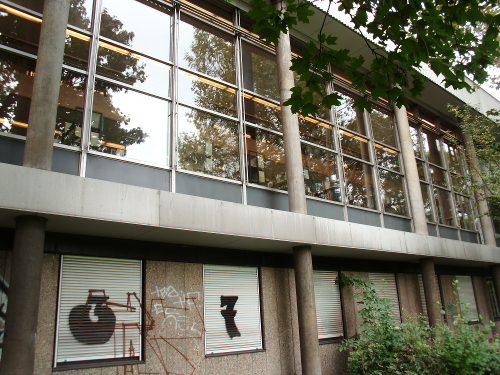
\includegraphics{./img/033.jpg}
\caption{Universitätsbibliothek Stuttgart (Stuttgart,
Deutschland)}
\end{figure}

\begin{figure}[htbp]
\centering
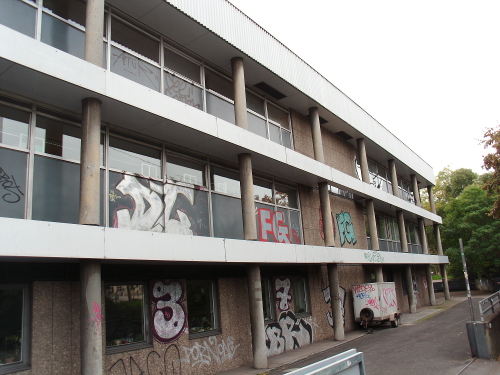
\includegraphics{./img/034.jpg}
\caption{Universitätsbibliothek Stuttgart (Stuttgart,
Deutschland)}
\end{figure}

\begin{figure}[htbp]
\centering
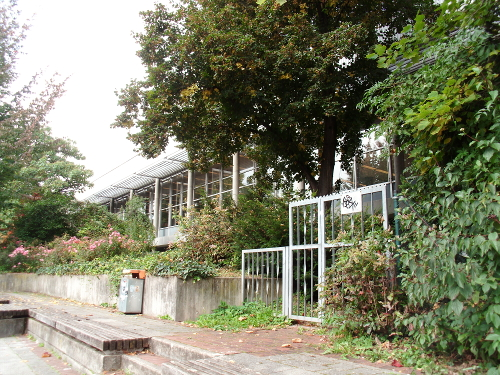
\includegraphics{./img/035.jpg}
\caption{Universitätsbibliothek Stuttgart (Stuttgart,
Deutschland)}
\end{figure}

\begin{figure}[htbp]
\centering
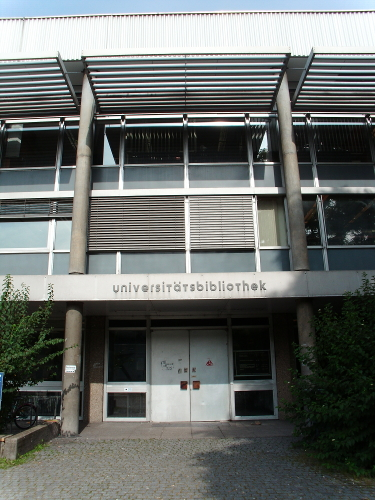
\includegraphics{./img/036.jpg}
\caption{Universitätsbibliothek Stuttgart (Stuttgart,
Deutschland)}
\end{figure}

\begin{figure}[htbp]
\centering
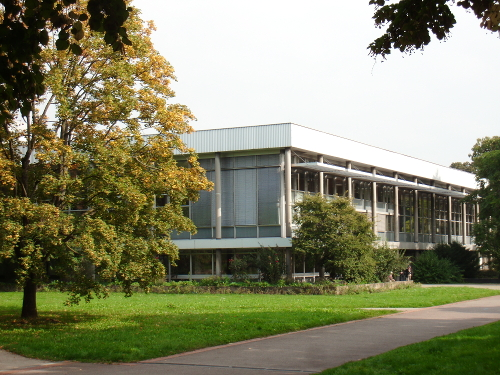
\includegraphics{./img/037.jpg}
\caption{Universitätsbibliothek Stuttgart (Stuttgart,
Deutschland)}
\end{figure}

\subsection*{Universitätsbibliothek Wien, Hauptbibliothek (Wien,
Österreich)}\label{universituxe4tsbibliothek-wien-hauptbibliothek-wien-uxf6sterreich}

\begin{quote}
\enquote{Der Wiederaufbau Österreichs nach dem Zweiten Weltkrieg stellte
die Universitäts\-bibliothek vor die Notwendigkeit, die verlagerten
Bestände wieder zurückzuführen und neue Wege zu finden, der gesteigerten
Hörer- und Benützerzahl gerecht zu werden. Nachdem das Projekt einer
neuen Universitätsbibliothek auf dem Areal des ehemaligen
Stadtkommandogebäudes (jetzt des neuen Institutsgebäudes) nicht
verwirklicht werden konnte {[}\ldots{}{]}, musste nun eine
durchgreifende Erneuerung und Erweiterung -- soweit dies im Rahmen des
bestehenden Gebäudes möglich war -- erfolgen. Um die Stellraumsituation
(Jahreszuwachs etwa 25.000 Bücher) zu erleichtern, musste der
Speicherraum wesentlich erweitert, ferner die Vorzone der Bibliothek
räumlich übersichtlicher gestaltet, entsprechend Raum für
Auskunftsdienst, Kopierstelle, sonstige Serviceeinrichtungen und vor
allem für einen zusätzlichen Lesesaal und einen neuen Zeitschriften- und
Zeitungslesesaal gewonnen werden. Als Kern der Anlage blieb der
Hauptlesesaal bestehen, doch wurde der Boden um 2 m gehoben, um
Verwaltungs- und Magazinsraum zu gewinnen.} (Jaksch, Fischer \& Kroller
1986, S. 64)
\end{quote}

\begin{quote}
\enquote{Die Benützerzahlen der Bibliothek stiegen sprunghaft an, sodaß
es nicht mehr mög\-lich war, für die personell aufwendige Garderobe (sechs
Personen pro Tag) Bibliotheksbedienstete bereitzustellen. {[}\ldots{}{]}
Daher mußte man sich zur Neuplanung der Garderobe entschließen.
{[}\ldots{}{]} Der hiefür {[}sic!{]} einzig geeignete Ort war, sowohl
raum- als auch funktionsgemäß, das Büchermagazin unter dem
Hauptlesesaal.} (Jaksch, Fischer \& Kroller 1986, S. 68)
\end{quote}

\begin{figure}[htbp]
\centering
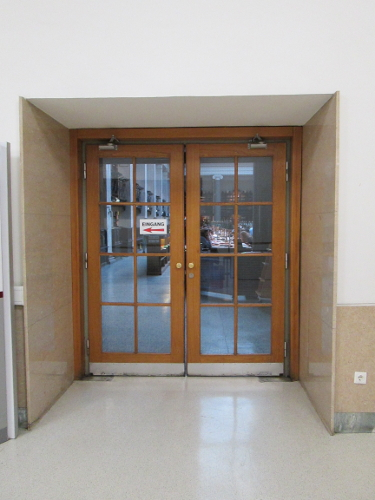
\includegraphics{./img/038.jpg}
\caption{Universitätsbibliothek Wien, Hauptbibliothek (Wien,
Österreich)}
\end{figure}

\begin{figure}[htbp]
\centering
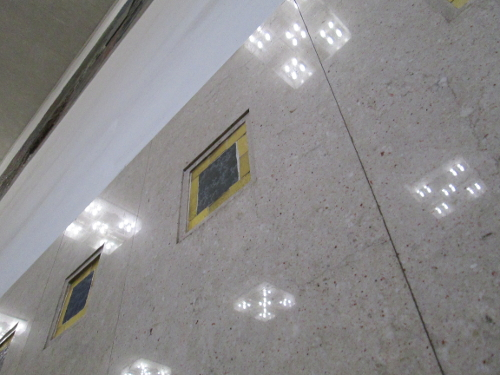
\includegraphics{./img/039.jpg}
\caption{Universitätsbibliothek Wien, Hauptbibliothek (Wien,
Österreich)}
\end{figure}

\begin{figure}[htbp]
\centering
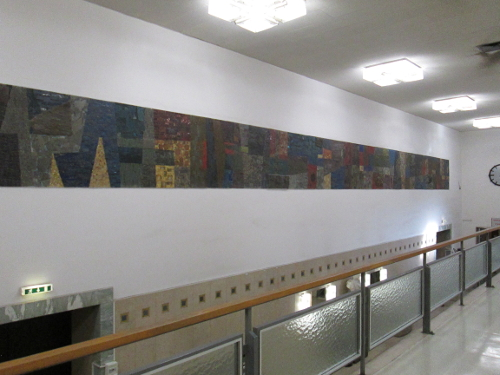
\includegraphics{./img/040.jpg}
\caption{Universitätsbibliothek Wien, Hauptbibliothek (Wien,
Österreich)}
\end{figure}

\begin{figure}[htbp]
\centering
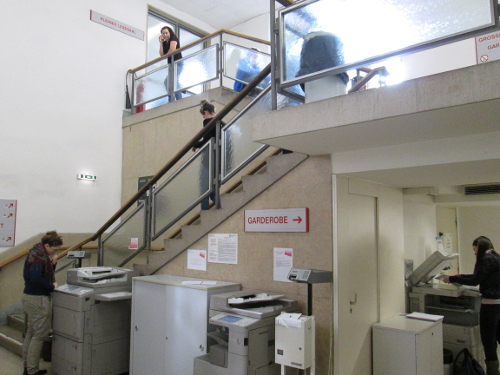
\includegraphics{./img/041.jpg}
\caption{Universitätsbibliothek Wien, Hauptbibliothek (Wien,
Österreich)}
\end{figure}

\subsection*{Universitätsbibliothek der Technischen Universität Wien
(Wien,
Österreich)}\label{universituxe4tsbibliothek-der-technischen-universituxe4t-wien-wien-uxf6sterreich}

\begin{quote}
``In den letzten Jahrzehnten wurden auf dem Gebiet des Bibliothekswesens
große Anstrengungen unternommen, um die Bibliotheken zu modernen
Dienstleistungsbetrieben im Rahmen eines leistungsfähigen,
wissenschaftlichen Informationswesens auszugestalten. Der Einsatz
moderner Techniken und Methoden und eine enge Zusammenarbeit aller
Bibliotheken sind das geeignete Mittel, um der Literaturflut und der
Bildungsexplosion Herr zu werden. Die Universitätsbibliothek der
Technischen Universität Wien ist daher auch mit allen modernen Geräten
und Einrichtungen ausgestattet, die einen rationellen Bibliotheksbetrieb
möglich machen. In Kürze wird die Bibliotheksverwaltung und -benützung
mit Hilfe der elektronischen Datenverwaltung erfolgen.
\end{quote}

\begin{quote}
Die neue Bibliothek ist also für die Zukunft gerüstet und wird imstande
sein, wissenschaftliches Arbeiten in hohem Maß zu unterstützen." (Tuppy
1988, S. 11)
\end{quote}

\begin{quote}
\enquote{Dieser schon äußerst dringlich gewordene Bibliotheksneubau der
Technischen Universität Wien ist ein städtebaulich wichtiger Beitrag zur
Schließung dieser Ecke am Karlsplatz, in dessen Ensemble er sich
einzufügen hat. Gleichzeitig soll er den formalen, technischen und
funktionellen Bedürfnissen unserer Zeit entsprechen.} (Jaksch, Fischer
\& Kroller 1986, S. 99)
\end{quote}

\begin{figure}[htbp]
\centering
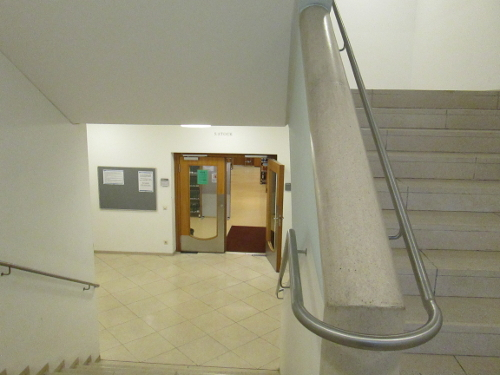
\includegraphics{./img/042.jpg}
\caption{Universitätsbibliothek der Technischen Universität Wien
(Wien,
Österreich)}
\end{figure}

\begin{figure}[htbp]
\centering
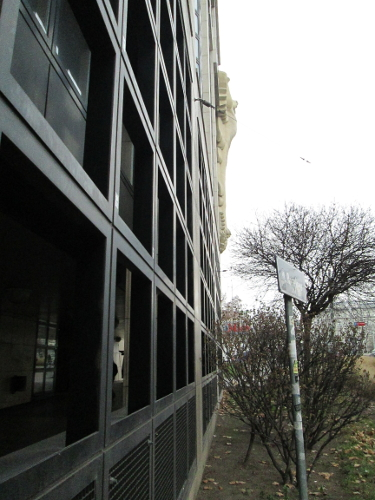
\includegraphics{./img/043.jpg}
\caption{Universitätsbibliothek der Technischen Universität Wien
(Wien,
Österreich)}
\end{figure}

\begin{figure}[htbp]
\centering
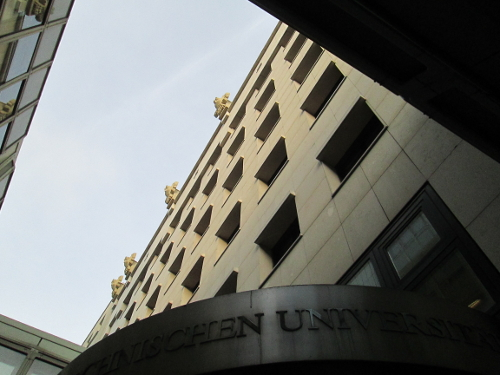
\includegraphics{./img/044.jpg}
\caption{Universitätsbibliothek der Technischen Universität Wien
(Wien,
Österreich)}
\end{figure}

\begin{figure}[htbp]
\centering
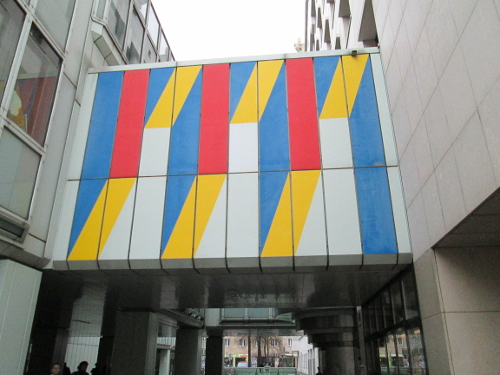
\includegraphics{./img/045.jpg}
\caption{Universitätsbibliothek der Technischen Universität Wien
(Wien,
Österreich)}
\end{figure}

\begin{figure}[htbp]
\centering
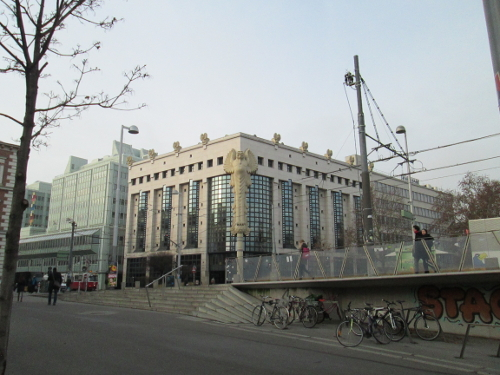
\includegraphics{./img/046.jpg}
\caption{Universitätsbibliothek der Technischen Universität Wien
(Wien,
Österreich)}
\end{figure}

\subsection*{Fakultätsbibliothek für Rechtswissenschaften an der
Universität Wien \enquote{Juridicum} (Wien,
Österreich)}\label{fakultuxe4tsbibliothek-fuxfcr-rechtswissenschaften-an-der-universituxe4t-wien-juridicum-wien-uxf6sterreich}

\begin{quote}
``Zur räumlichen Entlastung des Hauptgebäudes der Universität Wien wurde
im Jahre 1970 ein neues Gebäude für die Fakultät für
Rechtswissenschaften geplant und im Jahre 1974 mit dem Bau begonnen.
{[}\ldots{}{]}
\end{quote}

\begin{quote}
Diese Aufgabe war infolge der verhältnismäßig geringen zur Verfügung
stehenden verbaubaren Fläche (2630 m²), der beengten Platzverhältnisse --
das Areal ist allseitig von Straßen mit Gebäuden aus der Gründerzeit
umgeben -- sowie in Folge des umfangreichen Raumprogrammes, der
Höhenbeschränkung in der Verbauung und der baupolizeilichen Vorschriften
ziemlich schwierig." (Jaksch, Fischer \& Kroller 1986, S. 74)
\end{quote}

\begin{quote}
\enquote{Auch die Lage, Anordnung und Funktion des gesamten
Bibliotheksbereiches ist durchaus ungewöhnlich. Die Planung erfolgte
nach eingehenden Studien zahlreicher Bibliotheken in Europa und Amerika
durch den Architekten zusammen mit dem Baubeauftragten der Fakultät,
Univ.-Prof.~Dr.~Günther Winkler, und entwickelte sich aus den besonderen
Erfordernissen, nach den Vorstellungen der Fakultät für
Rechtswissenschaften; bibliothekarische Fachleute wurden erst in einem
ganz späten Stadium beigezogen und konnten nur mehr auf einige Details
der Bauplanung sowie auf die Einrichtung Einfluss nehmen.} (Jaksch,
Fischer \& Kroller 1986, S. 74)
\end{quote}

\begin{quote}
\enquote{Das gesamte Erdgeschoss füllt (mit Ausnahme der beiden
Stiegenhallen samt je drei Aufzügen und den Toiletteanlagen {[}sic!{]})
eine einzige große, ringsum verglaste Halle mit einer Sitzlandschaft,
Liftfaßsäulen, Münzkopiergeräten und einer Rampe für die Behinderten,
die in das darüberliegende, galerieartige Zwischengeschoß mit seiner
Buffetzone und einer Reihe von Esstischen, mit Blick in die große Halle,
führt.} (Jaksch, Fischer \& Kroller 1986, S. 75)
\end{quote}

\begin{quote}
\enquote{Die Anordnung stellt eine Lösung dar, die sich erst wird
bewähren müssen. Die Verteilung der Bücher auf fünf Geschosse (abgesehen
vom Magazin im zweiten Untergeschoß) ruft eine gewisse räumliche
Zersplitterung hervor, ermöglicht jedoch eine fachspezifische Zuteilung
zu den einzelnen Instituten.} (Jaksch, Fischer \& Kroller 1986, S. 76)
\end{quote}

\begin{figure}[htbp]
\centering
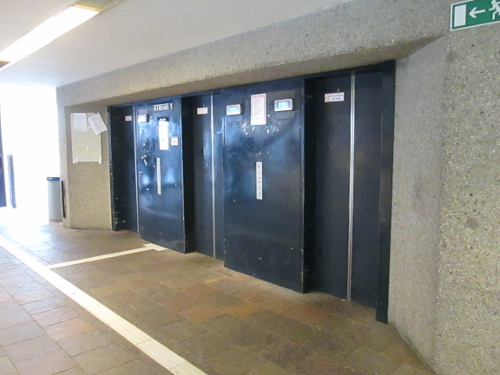
\includegraphics{./img/047.jpg}
\caption{Fakultätsbibliothek für Rechtswissenschaften an der
Universität Wien \enquote{Juridicum} (Wien,
Österreich)}
\end{figure}

\begin{figure}[htbp]
\centering
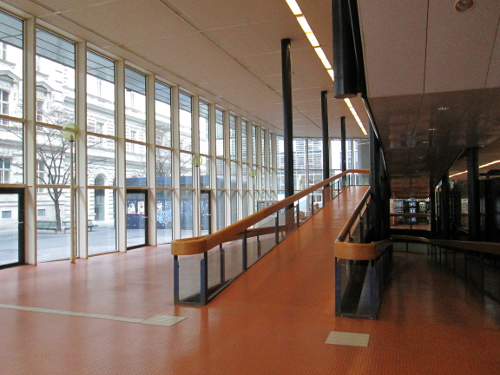
\includegraphics{./img/048.jpg}
\caption{Fakultätsbibliothek für Rechtswissenschaften an der
Universität Wien \enquote{Juridicum} (Wien,
Österreich)}
\end{figure}

\begin{figure}[htbp]
\centering
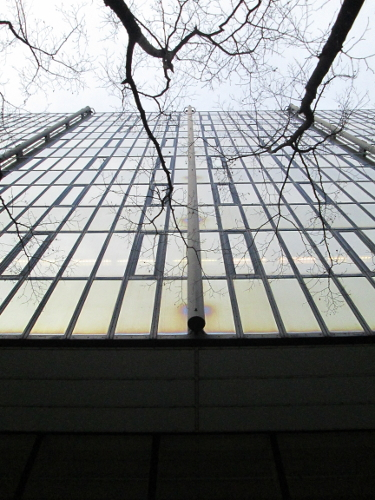
\includegraphics{./img/049.jpg}
\caption{Fakultätsbibliothek für Rechtswissenschaften an der
Universität Wien \enquote{Juridicum} (Wien,
Österreich)}
\end{figure}

\begin{figure}[htbp]
\centering
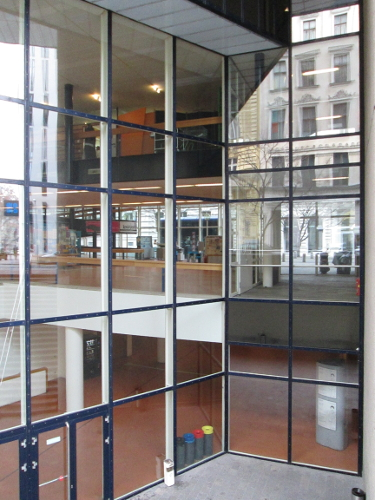
\includegraphics{./img/050.jpg}
\caption{Fakultätsbibliothek für Rechtswissenschaften an der
Universität Wien \enquote{Juridicum} (Wien,
Österreich)}
\end{figure}

\begin{figure}[htbp]
\centering
\includegraphics{./img/051.jpg}
\caption{Fakultätsbibliothek für Rechtswissenschaften an der
Universität Wien \enquote{Juridicum} (Wien,
Österreich)}
\end{figure}

\subsection*{Max-Planck-Institut für Bildungsforschung (Berlin,
Deutschland)}\label{max-planck-institut-fuxfcr-bildungsforschung-berlin-deutschland}

\begin{quote}
\enquote{Im Januar und Februar 1974 konnte der Neubau auf dem vom Land
Berlin der Max-Planck-Gesellschaft überlassenen Gelände am
Breitenbachplatz in Berlin bezogen werden. Er gilt als einer der
phantasievollsten Bauten der Berliner Nachkriegszeit und hat sich mit
seinem Konzept ‚von innen nach außen bauen‛ in den mehr als 6 Jahren
seiner Benutzung auch praktisch bewährt. In seiner Eingangshalle, die
durch die besondere Führung verschiedener Treppen und durch überraschend
gute Akustik dazu einlädt, finden zeitweilig auch Konzerte und
Ausstellungen von Bildern und Plastiken junger Künstler statt}
(Fuhltrott, Liebers \& Philipp 1983, S. 10)
\end{quote}

\begin{quote}
\enquote{Die Dokumentationsräume liegen mit dem übrigen Institut durch
die Eingangshalle verbunden in einem etwa sechseckigen Bauteil, der
einen kleinen, offenen, vorwiegend mit Schilfgewächsen bepflanzten
Innenhof einschließt. Dieser Innenhof wird ca {[}sic!{]} zur Hälfte
umgeben von dem 36 Plätze umfassenden Lesesaal, in dem zur Zeit die
laufenden Jahrgänge von 724 größtenteils ausländischen Zeitschriften in
Wandschränken ausliegen. Er wird erleuchtet durch die Glasfronten zum
Innenhof und durch runde Deckenfenster, die das Licht auf die
Zeitschriftenauslage lenken. Die Lesetische sind radial zum Innenhof
angeordnet und tragen in einer Sichtschutzwand verdeckte Neonröhren. Ein
Kopier-Gerät bietet in einem kleinen Nebenraum die Möglichkeit der
Fotokopie.} (Fuhltrott, Liebers \& Philipp 1983, S. 10)
\end{quote}

\begin{figure}[htbp]
\centering
\includegraphics{./img/052.jpg}
\caption{Max-Planck-Institut für Bildungsforschung (Berlin,
Deutschland)}
\end{figure}

\begin{figure}[htbp]
\centering
\includegraphics{./img/053.jpg}
\caption{Max-Planck-Institut für Bildungsforschung (Berlin,
Deutschland)}
\end{figure}

\begin{figure}[htbp]
\centering
\includegraphics{./img/054.jpg}
\caption{Max-Planck-Institut für Bildungsforschung (Berlin,
Deutschland)}
\end{figure}

\begin{figure}[htbp]
\centering
\includegraphics{./img/055.jpg}
\caption{Max-Planck-Institut für Bildungsforschung (Berlin,
Deutschland)}
\end{figure}

\subsection*{Bezirksbibliothek Köpenick (Berlin,
Deutschland)}\label{bezirksbibliothek-kuxf6penick-berlin-deutschland}

Bei der Bezirksbibliothek Köpenick (heute Treptow-Köpenick, Berlin)
liegt der interessante Fall vor, dass die Planungen eines Gebäudes
erhalten sind, welches durch das heutige Gebäude fast vollständig
ersetzt wurde. Nicht nur die politische Situation -- die
Bezirksbibliothek Köpenick wurde in der DDR geplant und gebaut --,
sondern auch die baulichen Möglichkeiten und Anforderungen haben sich
radikal geändert.

\begin{quote}
``Die Stadtbezirksbibliothek Berlin-Köpenick ist als Freihandbibliothek
mit einem kleinen Magazinbestand angelegt.
\end{quote}

\begin{quote}
Die Vorgabe, Altbauten auf zwei Seiten des Schüßlerplatzes ganz oder
teilweise einer neuen Nutzung zuzuführen, den Neubauanteil möglichst
gering zu halten, bedingt die räumliche Trennung einiger
Funktionsbereiche der Bibliothek.
\end{quote}

\begin{quote}
Sie führt auch dazu, die nutzungsneutrale Zone auf ein Mindestmaß, die
Erwachsenenbibliothek, zu beschränken und die Verteilung der übrigen
Raumgruppen nach ihrer Einordnungsfähigkeit in die vorhandenen
Baustrukturen und deren Deckenbelastbarkeit vorzunehmen. Dabei gilt es,
den Gesamtorganismus der Bibliothek mög\-lichst nicht bzw. nur gering zu
beeinträchtigen.
\end{quote}

\begin{quote}
An der Nordseite des Schüßlerplatzes, der Rosenstraße, liegen die
Erwachsenenbibliothek, die Kinderbibliothek, ein Lesecafe, die
Hausmeisterwohnung, ein Gäste\-appar\-tement und die Arbeitsräume des
Hausgrafikers. An der Südseite, der Jäger\-srtaße, befinden sich die
Phonothek, die Artothek, die Diathek, der Vortragssaal und
Verwaltungsräume sowie eine kleine Hausbuchbinderei {[}\ldots{}{]}.
\end{quote}

\begin{quote}
Von der Eingangshalle Rosenstraße 19 {[}\ldots{}{]} mit Kleiderablage
und Besucher-WC, im Bedarfsfall können die WCs der oberen Geschosse
mitbenutzt werden, gelangt der Leser sowohl über ein paar Stufen hinauf
zur Leihstelle als auch über wenige Stufen hinab in das Leseespresso für
die Tages- und Wochenpresse. Das Selbstbedienungslesecafe ist morgens,
bevor die Bibliothek für Leser geöffnet ist, der Frühstücksraum der
Mitarbeiter. Die Inseltheke für Ausleihverbuchung, Bücherausgabe und
-rück\-nah\-me, Anmeldung und Auskunft bildet zugleich die Speere. In ihrem
Blickfeld befindet sich der Sondereingang für Rollstuhlfahrer, die auf
dieser Ebene ihre Buch\-wünsche selbst erfüllen können oder sonst von
Bibliotheksmitarbeitern bedient werden.
\end{quote}

\begin{quote}
Das Thekenrund trennt die Zugänge zur Kinder- und zur
Erwachsenenbibliothek. Die Ausleihverbuchung geschieht mittels Handleser
für Zeichenerkennung (``Lesepistolen) {[}sic!, keine abschliessenden
Zeichen{]}, die mit zwei Kleincomputern verbunden sich. Die Belege
werden von einem Mosaikdrucker ausgefertigt.
\end{quote}

\begin{quote}
Ein Kleinlastenaufzug verbindet die Leihstelle mit dem Kellermagazin und
dem Rücksortierraum mit Xerografiestelle im Obergeschoß.
\end{quote}

\begin{quote}
Die drei Ebenen der Kinderbibliothek bieten den Bestand
altersstufengemäß dar. Die gläserne Fassade öffnet sich zum Garten, der
für Lesungen, Spiele und dgl. benutzt werden kann. Übrigens können sich
die jungen Leser in Thekennähe die Hände waschen. Das Eingangsgeschoß
der Erwachsenenbibliothek hält Zeitschriften und den Informationsbestand
bereit. Im Obergeschoß werden Kataloge, Information, Belletristik und
der Sachbuchbestand plaziert. Ihnen ist die Vervielfältigungsstelle
zugestellt. In diesem nutzungsneutralen Großraum kann die
Aufstellungsform leicht verändert werden. Er genügt
Flexibilitätsansprüchen.
\end{quote}

\begin{quote}
Die Obergeschosse des Hauses Rosenstraße 19 nehmen die Abteilung
Literaturpropaganda, die Leitung der Hauptbibliothek und der
Frauenruheraum ein; das Untergeschoß den Hausanschluß und die
selbsttätige Telefonzentrale auf. Das Obergeschoß des Hauses Rosenstraße
17 beherbergt die Dreiraumwohnung des Hausmeisters und ein
Gästeappartement.
\end{quote}

\begin{quote}
Auf der Platzseite gegenüber befinden sich im Erdgeschoß des Hauses
Jägerstraße 1\,-\,2 Phonothek {[}\ldots{}{]}, Artothek und Diathek in
einem Raum. In die Verbuchungstheke ist ein zentraler Abspieltisch
eingebaut. Musikliteratur und Schallplatten werden vorwiegend in
Freihandaufstellung angeboten. Gepolsterte Sitzstufen gestatten ein
entspanntes, bequemes Hören mit Blick auf den Hinterhof.
\end{quote}

\begin{quote}
Die Bilder der Artothek sind in einem Schaudepot gespeichert. Die
aufgeblockten Reproduktionen werden an den Drahtgittern herausziehbarer,
raumhoher Stahlrahmen befestigt.
\end{quote}

\begin{quote}
Der Vortragssaal im zweiten Obergeschoß {[}\ldots{}{]} ist mit einer
Studioanlage ausgestattet. Die übrigen Räume beider Obergeschosse sind
hauptsächlich für die Direktion, die allgemeine Verwaltung und das
Lehrkabinett bestimmt. Teeküche und sanitäre Anlagen bilden notwendige
Ergänzungen.
\end{quote}

\begin{quote}
Die Heizungsanlage, sie wird wahrscheinlich später zu einer
Umformerstation der Fernwärmeversorgung umgerüstet, liegt wegen der
erforderlichen Schornsteinhöhe im Haus Jägerstraße 1 - 2. Der hohe
Grundwasserspiegel verbietet einen unterirdischen Kohlenbunker. Der
geringe Abstand zwischen Vorderhaus und Hintergebäude Kietzer Straße 7
verhindert die Durchfahrt von Lastkraftwagen zum Innenhof dieses Hauses.
Daher muß das Brennstofflager vom Schüßlerplatz aus ebenerdig beschickt
werden. Kleine Belieferungsfahrzeug vom Typ Multicar können
hineinfahren. Größere rollen an das Gebäude heran und kippen die
Briketts in den Bunker, der durch ein Rolltor verschlossen wird. Die
Aschekübel gelangen über einen Ascheaufzug auf den Innenhof und werden
in einem Ascheraum des Hinterhauses Kietzer Straße 7 zwischengelagert.
Dieser Raum nimmt auch die Mülltonnen der Wohnungen der Gebäude
Jägerstraße 3 - 3a und Kietzer Straße 7 auf.
\end{quote}

\begin{quote}
Im Eingangsgeschoß des Hauses Jägerstraße 3 - 3a {[}\ldots{}{]} arbeiten
die Erwerbungs- und Katalogisierungsabteilung, sie verfügt über einen
Dienstkatalog, und benachbart, die Hausbuchbinderei. Den Geschäftsgang
durchlaufen auch die Neuerwerbungen für die Zweigstellen." (Prohl 1985,
S. 16ff.)
\end{quote}

\begin{figure}[htbp]
\centering
\includegraphics{./img/056.jpg}
\caption{Bezirksbibliothek Köpenick (Berlin,
Deutschland)}
\end{figure}

\begin{figure}[htbp]
\centering
\includegraphics{./img/057.jpg}
\caption{Bezirksbibliothek Köpenick (Berlin,
Deutschland)}
\end{figure}

\begin{figure}[htbp]
\centering
\includegraphics{./img/058.jpg}
\caption{Bezirksbibliothek Köpenick (Berlin,
Deutschland)}
\end{figure}

\subsection*{Bibliothek Spiez (Spiez,
Schweiz)}\label{bibliothek-spiez-spiez-schweiz}

\begin{quote}
``\textbf{\emph{Der Bibliotheks-Pavillon}}
\end{quote}

\begin{quote}
Im Kanton Bern ist es eine der ersten freistehenden Bibliotheken: Ein
Leichtbaupavillon im Elementbau. Er steht im ehemaligen Schulgarten
zwischen Sekundarschulhaus und Gemeindehaus. Ungefähre Kosten: Gebäude
Fr. 205000.-, Inneneinrichtungen Fr. 65000.-. Während das Gebäude von
aussen mit seinen Eternitwänden eher etwas kahl aussieht, ist es dank
der Hilfe von Innenarchitekt Max Kräuchi gelungen, im Innern einen
sympathisch wirkenden Raum zu schaffen. Auf die Kinder wirken die
Sitzstufen sehr anziehend, die Erwachsenen setzten sich gerne in die
Fauteuils, um in einem Buch zu schmökern." (Schweizer Bibliotheksdienst
1980, ohne Seite)
\end{quote}

\begin{quote}
``\textbf{\emph{Ein bisschen Stolz}}
\end{quote}

\begin{quote}
Nach so langer Wartezeit {[}1967 Gründung der Freihandbibliothek durch
Zusammenschluss von Gemeinnütziger Gesellschaft Spiez und
Arbeiterbildungsausschuss -- 1980 Eröffnung des Pavillons{]} ist es
begreiflich, dass wir heimlich doch ein bisschen stolz sind auf unsere
Bibliothek; hat sich doch das hässliche kleine Entelein zu einer schönen
Ente -- (noch nicht zu einem stolzen Schwan!) -- durchgemausert. Das
zeigt sich an verschiedenen Details:
\end{quote}

\begin{itemize}
\itemsep1pt\parskip0pt\parsep0pt
\item
  Bibliothek Spiez
\end{itemize}

\begin{quote}
Wir nennen uns nicht mehr \enquote{Freihandbibliothek}, sondern bloss noch
\enquote{Bibliothek Spiez}, gibt es doch nur eine solche, die den Namen wirklich
verdient!
\end{quote}

\begin{itemize}
\itemsep1pt\parskip0pt\parsep0pt
\item
  Signet
\end{itemize}

\begin{quote}
Wie jede bessere Firma haben wir (nach unbefriedigenden eigenen
Veruschen) ein Signet durch Herrn Urs Gerber, Grafiker, Spiez, entwerfen
lassen. Es schmückt Briefbogen, Briefumschläge, Zeitungsartikel, Plakate
usw.
\end{quote}

\begin{itemize}
\itemsep1pt\parskip0pt\parsep0pt
\item
  Buchzeichen
\end{itemize}

\begin{quote}
Das einfache Buchzeichen aus Umweltschutz-Halbkarton wurde zu einem
Bestseller, sind doch die Benützer froh zu wissen, wann die Bibliothek
geöffnet ist -- und wo sie beim Lesen verblieben sind." (Schweizer
Bibliotheksdienst 1980, ohne Seite)
\end{quote}

\begin{figure}[htbp]
\centering
\includegraphics{./img/059.jpg}
\caption{Bibliothek Spiez (Spiez,
Schweiz)}
\end{figure}

\begin{figure}[htbp]
\centering
\includegraphics{./img/060.jpg}
\caption{Bibliothek Spiez (Spiez,
Schweiz)}
\end{figure}

\begin{figure}[htbp]
\centering
\includegraphics{./img/061.jpg}
\caption{Bibliothek Spiez (Spiez,
Schweiz)}
\end{figure}

\begin{figure}[htbp]
\centering
\includegraphics{./img/062.jpg}
\caption{Bibliothek Spiez (Spiez,
Schweiz)}
\end{figure}

\subsection*{Gemeindebibliothek Münsingen, Kornhaus Bibliotheken Bern
(Münsingen,
Schweiz)}\label{gemeindebibliothek-muxfcnsingen-kornhaus-bibliotheken-bern-muxfcnsingen-schweiz}

\begin{quote}
``\textbf{\emph{1971/72: Der grosse Durchbruch}}
\end{quote}

\begin{quote}
Mit dem Bau des neuen Schulhauses Schlossmatte begann der grosse
Durchbruch. Nun stand ein -- wie uns damals schien -- genügend grosser
Bibliotheksraum zur Verfügung. Zudem stimmte der Gemeinderat einem
Ausbauplan zu und bewilligte die Mittel für die Einrichtung einer
modernen Freihandbibliothek, deren Trägerin nach wie vor die
Bibliotheksgesellschaft Münsingen blieb. 1971 begann der Auszug aus dem
alten Raum im Schulhaus Mittelweg, und am 28. Januar 1972 konnte die
neue Freihandbibliothek eröffnet werden, fast auf den Tag genau 100
Jahre nach Gründung der Bibliotheksgesellschaft Münsingen!
\end{quote}

\begin{quote}
Noch immer war unsere Bücherei eine reine Erwachsenenbibliothek. Ende
Juni 1974 konnte dann eine Kinder- und Jugendabteilung angegliedert
werden, die so regen Zuspruch fand, dass bei der Bücherausgabe ein
Rationierungssystem eingeführt werden musste. Der 1975 auf 1500 Bände
angewachsene Bestand an Jugendbüchern wurde jährlich zwölfmal umgesetzt.
Die auf insgesamt 4500 Bände erweiterte Bücherei war organisations- und
raummässig schon an die äusserste Grenze der Belastbarkeit gelangt.
\end{quote}

\begin{quote}
Inzwischen war aber im Kanton Bern einiges geschehen: Die kantonalen
Behörden setzten sich tatkräftig für die Förderung von
Gemeindebibliotheken ein, und der Gedanke, dass eine leistungsfähige
Bibliothek unabdingbar zur Infrastruktur einer lebendigen Gemeinde
gehört, begann sich allgemein durchzusetzen.
\end{quote}

\begin{quote}
\textbf{\emph{1975: Das Angebot der Kirchgemeinde}}
\end{quote}

\begin{quote}
Im Oktober 1975 bot die Kirchgemeinde der Bibliothek Gastrecht im heute
(August/September 1978) eröffneten grosszügig ausgebauten und
architektonisch reizvollen Dachgeschoss des neuen Kirchgemeindehauses
an.
\end{quote}

\begin{quote}
\textbf{\emph{1976: Die politische Gemeinde beschliesst}}
\end{quote}

\begin{quote}
An der Gemeindeversammlung vom 28. Juni 1976 bewilligten die Stimmbürger
-- ohne Gegenstimme! -- einen Kredit von 200000 Franken {[}Anmerkung:
Kredit bedeutet in der schweizerischen Politik einen nicht
zurückzuzahlenden Etat{]} für die Errichtung einer neuen Volks- und
Jugendbibliothek, deren Trägerorganisation nach wie vor die
altehrwürdige Bibliotheksgesellschaft Münsingen bleiben wird, in deren
Vorstand Vertreter von Kirchgemeinde und Einwohnergemeinde Einsitz
nahmen.
\end{quote}

\begin{quote}
So ist ein schönes Gemeinschaftswerk entstanden, ganz im Sinne der
wackeren Pfarrherren Molz und Ziegler, die vor mehr als hundert Jahren
wohl wussten, dass eine Gemeindebibliothek mehr zu sein hat als ein
totes Büchermagazin, nämlich ein Ort der Begegnung!" (Gafner 1983, Ohne
Seite)
\end{quote}

\begin{figure}[H]
\centering
\includegraphics{./img/063.jpg}
\caption{Gemeindebibliothek Münsingen, Kornhaus Bibliotheken Bern
(Münsingen,
Schweiz)}
\end{figure}

\begin{figure}[H]
\centering
\includegraphics{./img/064.jpg}
\caption{Gemeindebibliothek Münsingen, Kornhaus Bibliotheken Bern
(Münsingen,
Schweiz)}
\end{figure}

\begin{figure}[H]
\centering
\includegraphics{./img/065.jpg}
\caption{Gemeindebibliothek Münsingen, Kornhaus Bibliotheken Bern
(Münsingen,
Schweiz)}
\end{figure}

\begin{figure}[H]
\centering
\includegraphics{./img/066.jpg}
\caption{Gemeindebibliothek Münsingen, Kornhaus Bibliotheken Bern
(Münsingen,
Schweiz)}
\end{figure}

\newpage

\section*{Literatur}\label{literatur}

Allenspach, Christoph ; Schibig, Marco (2001) / \emph{Die Schweizerische
Landesbibliothek in Bern : Renovation und Erweiterung 1994-2001}. Baden
: Verlag Lars Müller

Anonym (1917) / \emph{Neubau der Zentralbibliothek Zürich : 30. April
1917}. Zürich : Aschmann \& Scheller, {[}1917{]}

Anonym (1931) / \emph{Die Schweizerische Landesbibliothek in Bern :
Einweihung am 31. Oktober 1931} (1931). Zürich : Gebr. Fretz A.G.,
{[}1931{]}

Anonym (1989) / Die Geschichte der Amerika-Gedenkbibliothek. In:
Feireiss, Kristin (Hrsg.): \emph{14x Amerika-Gedenkbibliothek :
Architekten aus den Vereinigten Staaten planen für Berlin ; Architects
from the United States planning for Berlin}. Berlin : Wilhelm Ernst \&
Sohn, 1989, S. 8-9

Corthésy, Bruno (2008) / \emph{Das Palais de Rumine in Lausanne}
(Schweizerischer Kunstführer GSK). Bern: Gesellschaft für Schweizerische
Kunstgeschichte, 2008

Denisjew, W.N. (1954) / Die Arbeit der Massenbibliothek. In: ders.:
\emph{Die sowjetische Massenbibliothek : Zwei Beiträge}. Leipzig :
Verlag für Buch- und Bibliothekswesen, 1954, S. 7-198

Drozd, Kurt Wolfgang Drozd (1978) / Funktionsbeschreibung des Neubaus
aus bibliothekarischer Sicht. In: Vesper, Ekkehart (Hrsg.):
\emph{Staatsbibliothek Preussischer Kulturbesitz : Festgabe zur
Eröffnung des Neubaus in Berlin}. Wiesbaden : Reichert, 1978, S. 179-191

Fabre, Xavier ; Speller, Vincent (2012) / Bibliothèques hybrides. In:
Petit, Christelle ; Bonnefoy, Franck (Hrsg.): \emph{Architecture et
bibliothèque: 20 ans de construction}. Villeurbanne : Presse de
l'enssib, 2012, S. 53-57

Feireiss, Kristin (Hrsg.) (1989) / \emph{14x Amerika-Gedenkbibliothek :
Architekten aus den Vereinigten Staaten planen für Berlin ; Architects
from the United States planning for Berlin}. Berlin : Wilhelm Ernst \&
Sohn, 1989

Fuhltrott, Rolf; Liebers, Gerhard; Philipp, Franz-Heinrich (Hrsg.)
(1983) / \emph{Bibliotheksbauten in der Bundesrepublik Deutschland
1968-1983} (Zeitschrift für Bibliothekswesen und Bibliographie,
Sonderheft, 39). Frankfurt am Main : Vittorio Klostermann, 1983

Gafner, Fritz (1983): 150 Jahre Bibliotheksgeschichte. In: Schweizer
Bibliotheksdienst (Hrsg.): \emph{Die neue Bibliothek: Volks- und
Jugendbibliothek Münsingen BE}. Bern: Schweizer Bibliotheksdienst, 1983,
ohne Seitenzählung

Huster-Braumann, Henriette (2011) / Maximilian Debus: Die
Universitätsbibliothek und ihre Schrift. In: Stephan, Werner (Hrsg.) ;
Rambach, Christiane ; Pertschi, Ottmar (bearb.): \emph{50 Jahre Neubau
Universitätsbibliothek Stuttgart 2011}. Stuttgart :
Universitätsbibliothek Stuttgart, 2011, 145-152

Jaksch, Walter ; Fischer, Edith ; Kroller, Franz (1986) /
\emph{Österreichischer Bibliotheksbau : Architektur und Funktion ; II.
Band 1945-1985}. Wien ; Köln ; Graz : Hermann Böhlaus Nachf., 1986

Lux, Claudia (2011) / Erinnerungen an die Vereinigung in der Zentral-
und Landesbibliothek Berlin. In: Baron, Günter ; Riese, Reimar (Hrsg.):
\emph{Wendezeit -- Zeitwende in deutschen Bibliotheken : Erinnerungen
aus Ost und West}. Berlin : BibSpider, 2011, 141-163

Moser, Fritz (1964) / \emph{Die Amerika-Gedenkbibliothek Berlin:
Entstehung, Gestalt und Wirken einer Öffentlichen Zentralbibliothek}
(Beiträge zum Buch- und Bibliothekswesen, 13). Wiesbaden: Otto
Harrassowitz, 1964

Moser, Fritz (1954) / \emph{Amerika-Gedenkbibliothek Berliner
Zentralbibliothek: Zur Eröffnung am 17. September 1954}. {[}Berlin{]}:
{[}Amerika Gedenkbibliothek{]}

Paščenko, Fedor Nikolaevič ; Schwarz Gerhard (Hrsg.) (1986) /
\emph{Grundlagen des Bibliotheksbaus : Bibliotheksgebäude}. München ;
New York ; London ; Paris : Saur, 1986

Ramcke, Rolf (1981) / Bibliotheksbau heute - aus der Sicht des
Architekten. In: Fuhlrott, Rolf (Hrsg.): \emph{Bibliothekbau heute :
Überarbeitete und ergänzte Fassung der Vortragsfolge vom Januar und
Februar 1980 aus Anlaß des Wettbewerbs für den Neubau der Badischen
Landesbibliothek in Karlsruhe} (Zeitschrift für Bibliothekswesen und
Bibliographie ; 33). Frankfurt am Main : Vittorio Klostermann, 1981, S.
61-67

Schweizer Bibliotheksdienst (Hrsg.) (1980) / \emph{Die neue Bibliothek:
Bibliothek Spiez}. Bern: Schweizer Bibliotheksdienst, 1980

Seydelmann, Gertrud (1973) / \emph{Dänischer Bibliotheksbau}
(Bibliotheksdienst, Beiheft ; 92). Berlin: Deutscher Bibliotheksverband,
Arbeitsstelle für das Bibliothekswesen, 1973

Stephan, Werner (Hrsg.) ; Rambach, Christiane ; Pertschi, Ottmar
(bearb.) (2011) / \emph{50 Jahre Neubau Universitätsbibliothek Stuttgart
2011}. Stuttgart : Universitätsbibliothek Stuttgart, 2011

Philipp, Klaus Jan (2011) / Die Universitätsbibliothek im
architekturgeschichtlichen Kontext. In:~Stephan, Werner (Hrsg.) ;
Rambach, Christiane ; Pertschi, Ottmar (bearb.): \emph{50 Jahre Neubau
Universitätsbibliothek Stuttgart 2011}. Stuttgart :
Universitätsbibliothek Stuttgart, 2011, 125-143

Prohl, Peter (1985) / Ein Entwurf für die Stadtbezirksbibliothek
Berlin-Köpenick : Adaptionen vorhandener Wohn- und Geschäftshäuser des
18. und 19. Jahrhunderts für Bibliotheksaufgaben in Verbindung mit
Ergänzungsbauten. In: Wirth, Eberhard (Redak.): \emph{Gothaer
Baugespräch 1984: Vorträge zum Bibliotheksbau und Bibliotheksbetrieb}.
Berlin: Methodisches Zentrum für wissenschaftliche Bibliotheken und
Informations- und Dokumentationseinrichtungen des Ministeriums für Hoch-
und Fachschulwesen, 1985, S. 12-27

Tuppy, Hans (1988) / {[}Geleitwort des Bundesministers für Wissenschaft
und Forschung{]}. In: Wawrosch, Josef (Hrsg.): \emph{Festschrift zur
Eröffnung des neuen Gebäudes des Universitätsbibliothek der Technischen
Universität Wien} (Biblos-Schriften, 145). Wien : Hammerl-Verlag, 1988,
11

Wirth, Eberhard (Redak.) (1985) / \emph{Gothaer Baugespräch 1984:
Vorträge zum Bibliotheksbau und Bibliotheksbetrieb}. Berlin:
Methodisches Zentrum für wissenschaftliche Bibliotheken und
Informations- und Dokumentationseinrichtungen des Ministeriums für Hoch-
und Fachschulwesen, 1985

Wisniewski, Edgar (1978) / Raumvision und Struktur : Gedanken über Hans
Scharouns Konzeption zum Bau der Staatsbibliothek. In: Vesper, Ekkehart
(Hrsg.): \emph{Staatsbibliothek Preussischer Kulturbesitz : Festgabe zur
Eröffnung des Neubaus in Berlin}. Wiesbaden : Reichert, 1978, S. 144-158

\newpage

%autor
\begin{center}\rule{3in}{0.4pt}\end{center}

\textbf{Karsten Schuldt}, Wissenschaftlicher Mitarbeiter am
Schweizerischen Institut für Informations\-wissen\-schaften, HTW Chur;
Redaktion LIBREAS. Library Ideas. Promotion am Institut für Bib\-liotheks-
und Informationswissenschaft, HU Berlin. Publikationen unter anderem zu
Schul- und Öffentlichen Bibliotheken.

\textbf{Eliane Blumer}, Assistante de recherche et d'enseignement an der
Haute école de gestion in Genf. Forscht zu Benutzerfreundlichkeit von
digitalen Bibliotheken und semantischen Suchmaschinen.

Leben und arbeiten in Lausanne, Chur, Genf und Berlin.

\end{document}
